\documentclass[12pt]{report} 
\usepackage{polski}
\usepackage[utf8]{inputenc}
\usepackage{scrextend} % addmargin https://tex.stackexchange.com/a/35939/50062
\usepackage{xcolor} % kolory, pewnie do usuniecia na koniec
\usepackage{glossaries} % skróty
\usepackage{listings} % listingi
\usepackage[hidelinks]{hyperref} % clickable toc and refs

%\usepackage[hyphens]{url}
\usepackage{graphicx}

\glstoctrue % add acronyms to TOC

\lstset{
  basicstyle=\ttfamily,
  columns=fullflexible,
  frame=single,
  breaklines=true,
  postbreak=\mbox{\textcolor{red}{$\hookrightarrow$}\space}
}
\renewcommand\lstlistlistingname{Spis listingów}

\title{Modelowanie jakości kodu źródłowego na podstawie danych gromadzonych w systemach kontroli wersji}


\author{Wojciech Frącz}

\makeglossaries

\newglossaryentry{api}{name=API, description={Application Programming Interface}}
\newglossaryentry{ast}{name=AST, description={Abstract Syntax Tree}}
\newglossaryentry{csv}{name=CSV, description={Comma Separated Values}}
\newglossaryentry{lstm}{name=LSTM, description={Long short-term memory}}
\newglossaryentry{nlp}{name=NLP, description={Natural Language Processing}}
\newglossaryentry{rnn}{name=RNN, description={Recurrent neural network}}
\newglossaryentry{scqm}{name=SCQM, description={Source Code Quality Model}}
\newglossaryentry{ascqm}{name=aSCQM, description={Absolute Source Code Quality Model}}
\newglossaryentry{rscqm}{name=rSCQM, description={Relative Source Code Quality Model}}
\newglossaryentry{srp}{name=SRP, description={Single Responsibility Principle}}
\newglossaryentry{vcs}{name=VCS, description={Version Control System}}

\begin{document}

\maketitle

\tableofcontents

\chapter{Wstęp}
\label{section:introduction} 

\textcolor{red}{Jakość kodu jest ważna, jest wiele metod ale dużo z nich wymaga czasu i ludzi. Chcielibyśmy cos z tym zrobić.}

\section{Motywacja i teza}
\textcolor{red}{Dlaczego chcę się tym zajmować: będzie szybciej, łatwiej, CR będzie chętnie wykonywane więc ogólna jakość wytwarzanego oprogramowania wzrośnie.}

Szczegółowa analiza dostępnych prac traktujących o omówionej tematyce skłoniła mnie do postawienia następującej tezy rozprawy:

\begin{addmargin}{1cm}
\textit{Opracowanie jakościowego modelu kodu źródłowego z użyciem technik uczenia maszynowego na podstawie danych gromadzonych w systemach kontroli wersji pozwoli na wykazanie większej trafności w rozpoznawaniu kodu niskiej jakości niż dostępne obecnie narzędzia wykorzystujące jego statyczną analizę.}
\end{addmargin}

\section{Zakres prac i wyzwania stawianie rozprawie}
\textcolor{red}{Jasne stwierdzenie, że w rozprawie ograniczam się do analizy jednego języka programowania i stworzone rozwiązanie porównuję do istniejących metryk. Mimo takiego ograniczenia i tak muszę skądś wziąć dane, sensownie je odfiltrować i przygotować, by wykonanie przedsięwzięcia w ogóle było możliwe. Muszę też jakoś uzyskać poprawną klasyfikację, a to wymaga czasu i ludzi.}

\section{Główne osiągnięcia rozprawy}
\textcolor{red}{systematyzacja metryk kodu, zidentfyikowanie commitów refaktoryzacyjnych, budowa modelu opartego o RNN identyfikującego zmiany w kodzie, wykorzystanie wyników w przykładowym narzędziu do gamifikacji przeglądów kodu, popularyzacja przeglądów, zebranie wiedzy ekspertowej w code.fracz.com}

\section{Struktura rozprawy}
\textcolor{red}{w rozdziale 1 blabla}


\chapter{Istniejące rozwiązania}

\textcolor{red}{Że jakość kodu jest ważna i przez to popularny temat. Jej utrzymywanie obniża koszty,
przyspiesza wdrażanie rozwiązań. Jak ja zapewniać?}

\section{Refaktoryzacja techniką zapewniania kodu wysokiej jakości}
\textcolor{red}{O tym, że kod "gnije", że trzeba go poprawiać, stosować wzorce. Że jest to czasochłonne i nie ma przyrostu funkcjonalności więc nie jest biznesowe.}

\section{Zapachy kodu, czysty kod}
\label{sec:existing:smells}
\textcolor{red}{Że są, że wskazują na potrzebę refaktoryzacji. Przykłady.}

\section{Metryki kodu}
\textcolor{red}{Że są, jakie są, referencje do papierów analizujących ich przydatność w klasyfikacji refaktoryzacji, cognitive complexity}

\section{Testy}
\textcolor{red}{O tym, że pozwalają zachować wysoką jakosc kodu, że bronią przed regresjami, że jest TDD. Ale że wymagają czasu. Mój model ich nie zastąpi.}



\section{Przeglądy kodu}
\textcolor{red}{O tym, że pozwalają zachować wysoką jakosc kodu, dużo referencji}

\section{Integracja metryk, testów i przeglądów kodu}
\textcolor{red}{Że jest np. Travis który buduje PR na githunbie i daje feedback. My chcemy dostarczyć model, który popchnie to o krok dalej - nie tylko informacje o tym że cós nie przeszło albo że complexity jest takie a takie, ale wyraźna sugestia: jest lepiej i możesz szybko sprawdzić lub jest gorzej, zwróc uwagę}
% * <dajda@agh.edu.pl> 2018-08-11T12:30:07.330Z:
% 
% PR na githubie - od czego jest skrót PR i co masz na myśli tutaj?
% 
% ^.
\section{Podsumowanie}
\textcolor{red}{Nie jest źle, jest sporo narzędzi do wspierania programistów, sami programiści są raczej świadomi korzyści płynących z utrzymywania kodu wysokiej jakości. ALe można im pomóc, by praca była przyjemniejsza i by mniej czasu spędzać na sprawdzaniu czy jest ok a więcej na kreatywnym tworzeniu.}


\chapter{Koncepcja jakościowego modelu kodu źródłowego - SCQM}
\label{ch:proj}

\textcolor{red}{Jak planuję rozwiązać problem? Potrzebuję model, który będzie patrzył na kod tak jak programista. Który będzie potrafił rozpoznać więcej niż zapachy kodu, więcej niż metryki.}

Do budowy jakościowego modelu kodu źródłowego (\gls{scqm} - Source Code Quality Model) nie można przygotować listy reguł czy symptomów, które pozwalają odpowiednio sklasyfikować kod. W ten sposób działają narzędzia, które opierają się na statycznej analizie kodu. \gls{scqm} ma analizować kod podobnie do programisty wykonującego przegląd kodu. Model ten musi więc wyjść poza sztywno ustalone wartości metryk lub zapachy kodu. Tylko pod warunkiem osiągnięcia takiego zachowania teza rozprawy może zostać dowiedziona, a co za tym idzie - zbudowany model \gls{scqm} może pomóc programistom wykonywać przeglądy kodu szybciej. Zadaniem jakościowego modelu będzie wstępna klasyfikacja kodu źródłówego lub wprowadzanej zmiany, by odpowiednio zasugerować miejsca w kodzie, którym należy poświęcić więcej uwagi. W tym rozdziale przedstawiono koncepcję rozwiązania postawionego problemu.

\section{Wymagania stawiane modelowi}
\label{sec:proj:requirements}
\textcolor{red}{Wejście: kod źródłowy, lub zmiana (kod źródłowy przed i po zmianie). Wyjście: klasyfikacja mówiąca o tym na ile dany kod byłby postrzegany przez programistę jako "czysty" lub w drugim przypadku - na ile dana zmiana byłaby postrzegana przez programistę jako poprawiająca jakość. Musi to działać szybko (szybciej, niż programista wykonuje CR - żeby to miało sens). Model powinno dać się dostarczyć w formie narzędzia, które da się zintegrować z istniejącymi systemami (czyli że to będzie Python a Python jest w każdej piwnicy itp więc jest super).}
Aby \gls{scqm} był użyteczny, musi potrafić działać na rzeczywistym kodzie źródłowym, lub musi dostarczać narzędzia, które bezpośrednio z kodu źródłowego są w stanie uzyskać pożądaną reprezentację. Nie można wymagać od programisty, by tworzył kod w jakiś specjalny sposób, np. poprzez pisanie odpowiednich komentarzy, adnotacji itp.

Narzędzie implementujące jakościowy model kodu źródłowego ma naśladować analizę kodu przez programistę wykonującego przegląd. Dlatego wynikiem takiej analizy powinna być również analogiczna do tej podejmowanej przez programistę - czy dany kod powinien być zaakceptowany i dołączony do projektu? Jeśli wprowadzana funkcjonalność jest poprawna oraz kod jest odpowiedniej jakości - odpowiedź powinna być twierdząca. Jeśli nie, osoba wykonująca przegląd kodu - a także \gls{scqm} - powinny zgłosić potrzebę wprowadzenia usprawnień do przeglądniętego kodu źródłowego. Opisywane rozwiązanie nie będzie sprawdzić pierwszego wspomnianego czynnika - czyli poprawności implementacji. To zadanie nadal pozostanie dla programisty sprawdzającego kod. \gls{scqm} natomiast sprawdzi, czy jakość zaprezentowanego kodu jest zgodna z założeniami.

Doprecyzowując: wynikiem analizy kodu źródłowego za pomocą jakościowego modelu powinna być klasyfikacja mówiąca o tym na ile danych kod byłby postrzegany przez programistę jako "czysty", lub w przypadku analizy zmiany kodu - na ile byłaby ona oceniona przez programistę jako zmiana poprawiająca jakość kodu.

Ważnym wymaganiem niefunkcjonalnym modelu powinna być jego przenośność i łatwość zastosowania w istniejących platformach wspierających przeglądy kodu. Wdrożenie narzędzia implementującego \gls{scqm} do jednej z tych platform wykracza poza ustalony zakrez rozprawy, jednak opis przeprowadzenia porównania klasyfikacji w celu udowodnienia tezy rozprawy nie powinien pozostawić wątpliwości jak wykorzystać stworozny model w dowolnym narzędziu.

Podsumowując, wymagania które powinien spełnić zaimplementowany jakościowy model kodu źródłowego można przedstawić w trzech punktach:

\begin{enumerate}
\item Analiza tego samego kodu źródłowego, który poddawany jest analizie podczas przeglądów kodu źródłowego.
\item Wynikiem jest klasyfikacja przeanalizowanego kodu jako kod wysokiej bądź niskiej jakości.
\item Implementacja modelu jest łatwa do uruchomienia i zaaplikowania do dowolnie wybranego kodu źródłowego we wspieranym języku programowania.
\end{enumerate}

\section{Ograniczenia modelu}
Pierwszym ograniczeniem modelu \gls{scqm} jest wybór analizowanego języka programowania. Jakościowy model będzie budowany dla języka Java. Model będzie wspierać tę wersję Javy, którą będzie wspierać wybrany parser języka użyty do przygotowania danych wejściowych (zob. sekcja \ref{sec:impl:ast}). W momencie pisania rozprawy jest to Java 10.

\textcolor{red}{... ? nie wiem co jeszcze. trzeba opisać ograniczenia nałożone potem}

\section{Opracowanie modelu}
\textcolor{red}{Opis i jakiś piękny diagram jak to sobie wyobrażam: na początku data harvesting z githuba, odpowiednie wybranie metod i odrzucenie śmieci, klasyfikacja przez ludzi. Równolegle: zbudowanie sieci neuronowej (tu chyba potrzebna pomoc od MK) obsługującej obydwa przypadki wyżej (1 kod i 2 kody). Jak mamy jedno i drugie to nauczenie sklasyfikowanymi danymi RNN}

Do implementacji jakościowego modelu kodu źródłowego zostaną użyte metody uczenia głębokiego. Zostaną podjęte próby przekazania do modelu wiedzy programisty na temat źródła jego decyzji o sklasyfikowaniu danego kodu jako kodu odpowiedniej bądź nieodpowiedniej jakości.

\subsection{Zgromadzenie odpowiednich danych wejśćiowych}
W każdym problemie, w którym pojawiają się metody uczenia głębokiego, etap przygotowania danych jest jednym z najważniejszych. To od nich zależy skuteczność uczenia a następnie trafność klasyfikacji.

Budowa modelu \gls{scqm} musi rozpocząć się od zgromadzenia wystarczająco dużej liczby przykładów kodu ocenianego jako kod wysokiej i niskiej jakości. Tylko wtedy będzie możliwość odkrycia wzorców, które programista podczas przeglądu rozpoznaje jako symptomy "czystego" kodu.

Sposób odnalezienia i przefiltorwania danych został opisany w sekcjach \ref{sec:impl:wybor-github} oraz \ref{sec:impl:identification-commits}.

\subsection{Przygotowanie wejścia dla modelu}
Jednym z założeń \gls{scqm} (zob. sekcja \ref{sec:proj:requirements}) jest możliwość bezpośredniej analizy kodu źródłowego. Bez wątpienia ten cel musi zostać osiągnięty przez odpowiednie przekształcenie analizowanego kodu źródłowego do formatu, który może być podany jako wejście modelu.

Sposób przygotowania wejścia opisano w sekcjach \ref{sec:impl:ast} oraz \ref{sec:impl:rnn-input}.

\subsection{Zebranie wiedzy ekspertowej}
Budowa modelu \gls{scqm} zakłada pozyskanie wiedzy ekspertowej od programistów. W ramach pracy nad rozprawą zostanie przeprowadzone badanie mające na celu zebranie opinii programistów na temat jakości kodu źródłowego.

Doświadczenie zostało dokładnie opisane w sekcji \ref{sec:impl:codefracz}. Będzie ono polegać na przedstawieniu programistom przykładów kodu realizującego podobne funkcjonalności, ale różniącego się jakością lub sposobem implementacji. Zadaniem programisty będzie wykonanie przeglądu obydwu przykładów i ocena, które z zaprezentowanych rozwiązań cechuje jego zdaniem wyższa jakość kodu.

Na podstawie badania autor rozprawy ma nadzieję wprowadzić do modelu \gls{scqm} rzeczywiste opinie programistów a co za tym idzie - podnieść końcową trafność i użyteczność opracowanych klasyfikacji.

\subsection{Implementacja modelu}
Posiadając odpowiednie dane wejściowe należy zaimplementować model, który będzie w stanie przyswoić wiedzę zawartą w zebranych przykładach kodu wysokiej i niskiej jakości.

Do tego celu została wybrana dwukierunkowa rekurencyjna sieć neuronowa (\gls{rnn}). Motywacja stojąca za wyborem tego rozwiązania oraz szczegóły implementacji zostały przedstawione w sekcji \ref{sec:impl:rnn}.

\subsection{Uczenie modelu}
Po zebraniu danych i zaimplementowaniu sieci neuronowej należy zbudować model wiedzy, który będzie potrafił sklasyfikować przykłady ze zbioru testowego oraz nowe przykłady metod, które nie znalazły się w zgromadzonym zbiorze danych.

Jak pokaże lektura rozdziału \ref{ch:learn}, w trakcie prób uczenia modelu podjęto szereg kolejnych decyzji poprawiających jakość danych wejściowych, ograniczając zebrane przykładu kodu, które nie wskazywały jednoznacznie jego jakości.

\subsection{Ewaluacja modelu}
Po skutecznym przekazaniu wiedzy do modelu \gls{scqm}, ostatnim krokiem prowadzącym do weryfikacji tezy rozprawy będzie porównanie klasyfikacji kodu źródłowego który nie został użyty do nauczenia modelu przez stworzony jakościowy model oraz dowolne inne narzędzie potrafiące dokonać statycznej analizy kodu.

Oczekuje się, że klasyfikator oparty o \gls{scqm} będzie trafniej rozpoznawać kod niskiej jakości. Wyniki ewaluacji przedstawiono w rozdziale \ref{ch:eval}.

\section{Model bezwględny aSCQM}
\label{sec:proj:bz}
Jakościowy model kodu źródłowego będzie zbudowany w dwóch wariantach. Pierwszy to wariant bezwzględny - \gls{ascqm} (Absolute Source Code Quality Model) - opisany w tej sekcji. Wariant względny - \gls{rscqm} (Relative Source Code Quality Model) - został opisany w sekcji \ref{sec:proj:wz}.

Model bezwzględny na wejściu dostaje jedną próbkę kodu źródłowego. Zadaniem modelu jest jej sklasyfikowanie, czyli wyznaczenie prawdopodobieństwa określającego szanse na to, że zadany kod jest kodem "czystym". Rysunek \ref{fig:proj:ascqm-s} przedstawia schemat działania modelu \gls{ascqm}. Na wejściu zadany jest kod źródłowy $S$ (od ang. "sample"). Wynikiem klasyfikacji są dwie liczby $P_G$ oraz $P_B$ przyjmujące wartości z zakresu $[0,1]$ oznaczające odpowiednio prawdopodobieństwa, że zadany kod jest wysokiej, bądź niskiej jakości. Oznaczenia $P_G$ oraz $P_B$ pochodzą z języka angielskiego - $G$ od ang. "good", oraz $B$ - "bad".

\begin{figure}
\centering
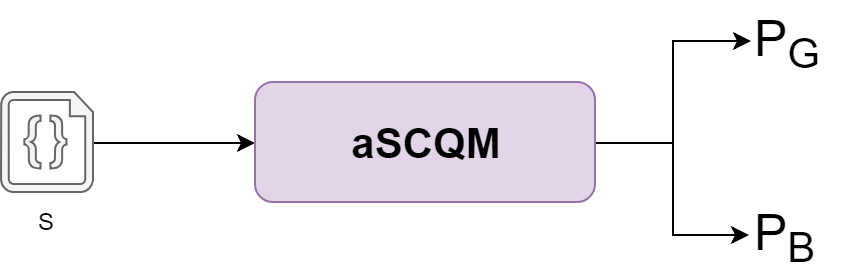
\includegraphics[width=\textwidth]{proj/ascqm-s.png}
\caption{Schemat działania modelu \gls{ascqm}.}
\label{fig:proj:ascqm-s}
\end{figure}

W trakcie uczenia modelu \gls{ascqm} na wejściu zostaną podane kolejno przykłady kodu wysokiej jakości ($G$) oraz kodu niskiej jakości ($B$). Do uczenia ze wzmocnieniem zostaną użyte odpowiednie wektory zawierające stuprocentowe prawdopodobieństwo odpowiedniego parametru - $P_G$ dla próbek pozytywnych oraz $P_B$ dla próbek negatywnych. Rysunki \ref{fig:proj:ascqm-g} oraz \ref{fig:proj:ascqm-b} zawierają proste schematy sposobu uczenia modelu \gls{ascqm}.

\begin{figure}
\centering
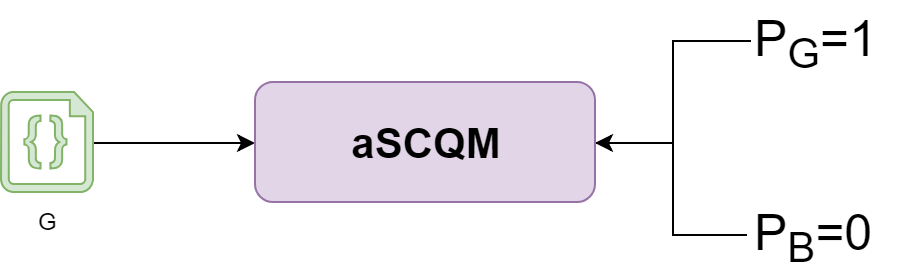
\includegraphics[width=\textwidth]{proj/ascqm-g.png}
\caption{Schemat uczenia modelu \gls{ascqm} - przypadek z kodem wysokiej jakości $G$ na wejściu}
\label{fig:proj:ascqm-g}
\end{figure}

\begin{figure}
\centering
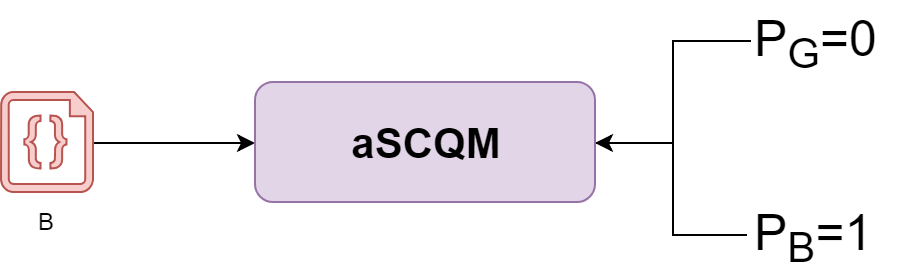
\includegraphics[width=\textwidth]{proj/ascqm-b.png}
\caption{Schemat uczenia modelu \gls{ascqm} - przypadek z kodem niskiej jakości $B$ na wejściu}
\label{fig:proj:ascqm-b}
\end{figure}

Model bezwzględny nie potrzebuje zmiany, która zaszła w kodzie źródłowym. Powinien on być w stanie sklasyfikować dowolny zadany kod źródłowy podobnie do programisty, który widzi dany kod po raz pierwszy. Model \gls{ascqm} stara się odpowiedzieć na pytanie:

\begin{quote}
\textbf{Czy przedstawiony kod jest kodem wysokiej jakości?}
\end{quote}

\section{Model względny rSCQM}
\label{sec:proj:wz}
Model względny ma za zadanie ocenić zmianę w kodzie źródłowym. Jest to ukłon w stronę zmian wprowadzanych w projekcie. Zdecydowana większość przeglądów kodu skupia się właśnie na ocenie wprowadzanej zmiany, a nie na klasyfikacji całego kodu źródłowego. Model \gls{rscqm} powinien więc być bardziej przydatny przy potencjalnej integracji jakościowego modelu z platformami wspierającymi przegląd kodu źródłowego.

W odróżnieniu od modelu bezwzględnego, na wejściu powinien on otrzymać dwie próbki kodu. Pierwsza z nich to postać kodu źródłowego przed zmianą a druga - po zmianie. Zadaniem modelu jest zwrócenie klasyfikacji oznaczającej prawdopodobieństwo, że dana zmiana podnosi jakość kodu źródłowego. Rysunek \ref{fig:proj:rscqm-ss} przedstawia schemat działania modelu \gls{rscqm}. Na wejściu zadana jest zmiana kodu źródłowego w postaci dwóch próbek $S_1$ i $s_2$ (od ang. "sample"), będące odpowiednio kodem źródłowym przed i po wprowadzonej zmianie. Wynikiem klasyfikacji są dwie liczby $P_G$ oraz $P_B$ przyjmujące wartości z zakresu $[0,1]$ oznaczające odpowiednio prawdopodobieństwa, że zadany zmiana podnosi lub obniża jakość kodu. Oznaczenia $P_G$ oraz $P_B$ pochodzą z języka angielskiego - $G$ od ang. "good", oraz $B$ - "bad".

\begin{figure}
\centering
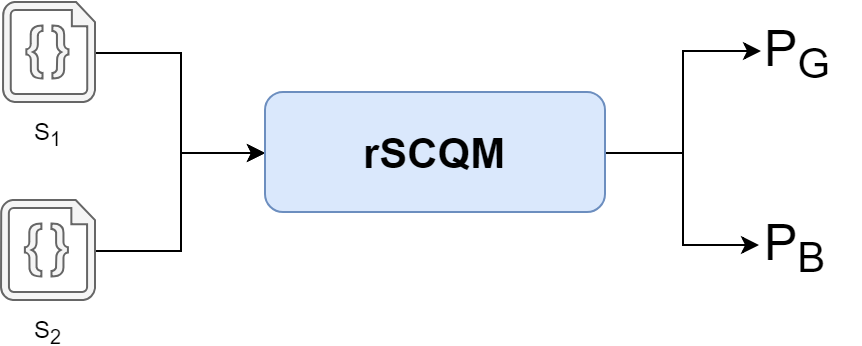
\includegraphics[width=\textwidth]{proj/rscqm-ss.png}
\caption{Schemat działania modelu \gls{rscqm}.}
\label{fig:proj:rscqm-ss}
\end{figure}

W trakcie uczenia modelu \gls{rscqm} na wejściu zostaną podane przykłady zmian kodu źródłowego. Z każdej zmiany zostanie wybrany kod wyższej jakości ($G$) oraz niższej jakości ($B$). Do uczenia ze wzmocnieniem zostaną użyte odpowiednie wektory zawierające stuprocentowe prawdopodobieństwo odpowiedniego parametru - $P_G$ dla zmian podnoszących jakość kodu ("gorsza" próbka $B$ podana jako pierwsza) oraz $P_B$ dla zmian, które ją pogarszają (próbka $B$ podana jako druga). Rysunki \ref{fig:proj:rscqm-bg} oraz \ref{fig:proj:rscqm-gb} zawierają proste schematy sposobu uczenia modelu \gls{rscqm}.

\begin{figure}
\centering
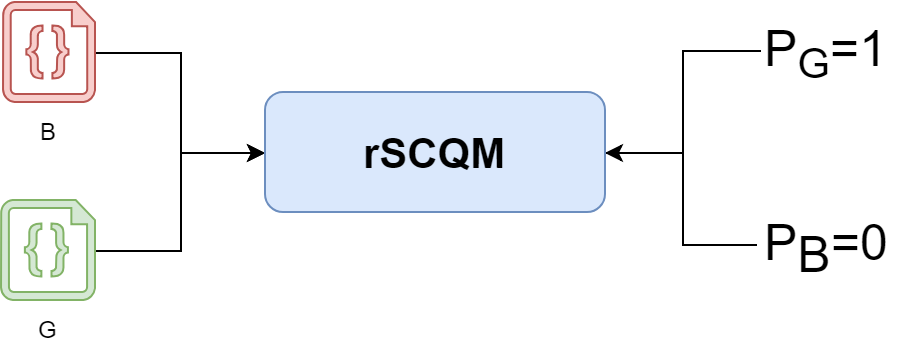
\includegraphics[width=\textwidth]{proj/rscqm-bg.png}
\caption{Schemat uczenia modelu \gls{rscqm} - przypadek ze zmianą poprawiająca jakość kodu}
\label{fig:proj:rscqm-bg}
\end{figure}

\begin{figure}
\centering
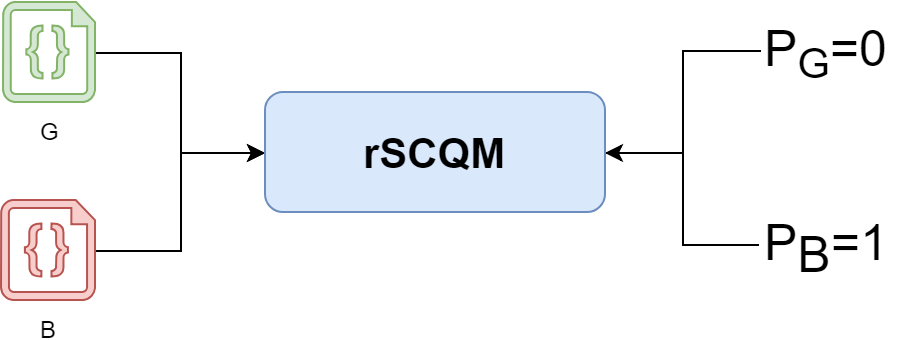
\includegraphics[width=\textwidth]{proj/rscqm-gb.png}
\caption{Schemat uczenia modelu \gls{rscqm} - przypadek ze zmianą pogarszającą jakość kodu}
\label{fig:proj:rscqm-gb}
\end{figure}

Model względny naśladuje programistę wykonującego przegląd kodu zmiany wprowadzanej do projektu. Stara się odpowiedzieć na pytanie:

\begin{quote}
\textbf{Czy wprowadzana zmiana podnosi jakość kodu źródłowego?}
\end{quote}

\section{Wykorzystanie modelu}
\textcolor{red}{Opis i jakiś piękny diagram jak to sobie wyobrażam:  wdrożenie: wykorzystanie nauczonego modelu w "życiu" a do celów rozprawy - wykorzystanie modelu do porównania mojeog rozwiązania z narzędziami do statycznej analizy kodu. Tutaj bez szczegółów "JAK" - to będzie dalej. Dzięki temu sprawdzę czy w ogóle ma to sens i dowiodę tezę.}

Jeśli zbudowany model wykaże większą trafność w klasyfikowaniu kodu wysokiej lub niskiej jakości, potwierdzi to postawioną w rozprawie tezę. To nie jest jednak głównym celem prowadzonych prac.

Model \gls{ascqm} będzie mógł być wykorzystywany do oceny jakości istniejącego kodu. To pozwoli np. na automatyczne porównanie wyników pracy różnych zespołów programistycznych. Dzięki takiemu rozwiązaniu można będzie nie tylko skupić się na efektach pracy programistów w postaci liczby napisanych linii kodu czy zamkniętych zadań, ale także na jakości dostarczanych przez nich rozwiązań. Takie narzędzie byłoby z pewnością docenione na szczeblu menedżerskim oraz osób odpowiedzialnych za zatrudnienie czy ewaluację pracy programistów.

Model \gls{rscqm} może mieć bardzo pozytywny wpływ na popularyzację praktyki przeglądów kodu źródłowego. Jak wykazano w \textcolor{red}{REF}, przeglądy kodu są niechętnie wykonywane przez programistów ze względu na ich czasochłonność i niski - w stosunku do tworzenia kodu - poziom kreatywności wykonywanej pracy. Sugestie o jakości proponowanych zmian od modelu względnego powinny przyspieszyć przegląd kodu dzięki sugerowaniu miejsc, na które należy zwrócić uwagę oraz tych, które można pominąć, gdyż automatyczna klasyfikacja nie wykazała w nich żadnych podejrzeń.

Integracja \gls{rscqm} z istniejącymi platformami wspierającymi przeglądy kodu powinna polegać na dostarczeniu mechanizmu, który po każdej nadesłanej zmianie, przed powiadomieniem osoby odpowiedzialnej za wykonanie przeglądu, poddaje proponowaną zmianę automatycznej klasyfikacji. \gls{rscqm} identyfikuje te zmiany, które pogarszają jakość kodu i zwraca informacje o nich do integrowanej platformy. Ta z kolei powinna wyświetlić w interfejsie użytkownika wskazane miejsca z informacją, że jakościowy model kodu źródłowego podejrzewa w nich istnienie problemów z jakością.

Integracja \gls{scqm} leży poza zakresem rozprawy, jednakże powyższy opis oraz dalsze szczegóły implementacji powinny jasno zarysować sposób jej ewentualnego przeprowadzenia.


\section{Podsumowanie}
Projekt jakościowego modelu kodu źródłowego \gls{scqm} oraz analiza jego dwóch wariantów - względnego i bezwzględnego - jasno zakreśla zakres prowadzonej rozprawy. Opisana metodologia powinna doprowadzić do uzyskania satysfakcjonujących wyników i otrzymania klasyfikatora jakości kodu źródłowego, który patrzy na kod "oczami programisty". Kolejne rozdziały rozprawy przedstawiają szczegóły implementacji \gls{scqm} oraz uzyskane rezultaty.

\chapter{Implementacja jakościowego modelu kodu źródłowego}
\label{ch:impl}

Dokładne zaplanowanie prac i zdefiniowanie oczekiwanych rezultatów w rozdziale \ref{ch:proj} pozwoliło na przystąpienie do implementacji przedstawionych założeń. W tym rozdziale opisano sposób zgromadzenia danych, za pomocą których model \gls{scqm} powinien posiąść pożądaną wiedzę oraz sposób ich przygotowania. Opisano także szczegółowo budowę sieci neuronowej odpowiedzialnej za klasyfikację oraz badanie, którego celem było pozyskanie jak największej i najdokładniejszej wiedzy ekspertowej na temat jakości kodu źródłowego.

\section{Źródło danych}
\textcolor{red}{Krótko o tym co to repozytorium i Git. Dlaczego github (bo popularny i otwarty), co to data harvesting, dlaczego tak (bo naszych projektów za mało, open source dużo).}

Naturalnym źródłem, z którego można pozyskać dane przy analizowaniu kodu źródłowego są repozytoria kodu otwartych projektów (ang. open source). Ich licencje pozwalają na bezpłatne zapoznanie się z kodem źródłowym, a zazwyczaj także na jego wykorzystanie lub nawet modyfikację. Nad kodem źródłowym otwartych projektów często pracuje też spora liczba programistów - szczególnie gdy bierzemy pod uwagę projekty popularne, używane przez znaczną liczbę użytkowników.

Te cechy powinny czynić z popularnych otwartych projektów doskonałe przykłady kodu, który jest kodem czystym i kodem wysokiej jakości. Skoro większość jego części była przeglądnięta przez kilku programistów, jest duża szansa że nie tylko jest on działający ale także zrozumiały czy czytelny. Niestety, sam wybór najpopularniejszych otwartych projektów nie pozwoliłby na zbudowanie jakościowego modelu kodu, bo nie można założyć, że sama otwartość i popularność projektu niesie ze sobą odpowiednią jakość w całym kodzie źródłowym.

Kod źródłowy przechowywany jest w repozytorium kodu źródłowego, zwanego też systemem kontroli wersji (ang. Version Control System, \gls{vcs}). W stosunku do zwykłego przechowywania plików na dysku, najważniejszą zaletą korzystania z repozytoriów kodu jest fakt, że oprócz przechowywania aktualnej wersji kodu, repozytorium przechowuje całą historię tworzenia danego projektu. Historia ta podzielona jest na kolejne zmiany (ang. commit), które jeden po drugim tworzą pełną historię stworzenia projektu od pierwszego pliku aż po stan na dzień dzisiejszy.

Jednym z najpopularniejszych systemów kontroli wersji w momencie pisania rozprawy jest Git. Jest to system darmowy i bardzo funkcjonalny, pozwalający na łatwe zarządzanie kodem projektu. Z tego powodu jest on bardzo często wybierany jako system kontroli wersji dla otwartych projektów.

Przykładem popularnej platformy, która udostępnia darmowe repozytoria Git do przechowywania repozytoriów otwartych projektów jest GitHub. W celu pozyskania danych, które pozwolą na zbudowanie \gls{scqm} w pracy nad rozprawą wykorzystano popularne repozytoria kodu źródłowego Git przechowywane na platformie GitHub.


\subsection{Wybór repozytoriów kodu}
\label{sec:impl:wybor-github}
\textcolor{red}{Że TOP 300 po gwiazdkach a nie po rozmiarze, bo gwiazdki oznaczają popularność projektu a jak cos jest popularne to może tam dbają o jakość. No i że Java. Zapytanie do githuba które mi wybrało te projekty. Lista TOP 10.}

GitHub, poza udostępnieniem możliwości darmowego przechowywania repozytoriów kodu otwartych projektów, oferuje także funkcjonalności, które umożliwiają zbudowanie społeczności wokół nich. Jednym z takich mechanizmów jest mechanizm oznaczania przez użytkowników wybranych projektów gwiazdkami. W dokumentacji GitHuba\footnote{\url{https://help.github.com/articles/about-stars/}} możemy przeczytać, że celem tej funkcjonalności jest możliwość oznaczenia interesujących projektów tak, by można je było potem szybciej odnaleźć. Przekazanie gwiazdki przez użytkownika oznacza także docenienie pracy włożonej w projekt przez jego autorów, a sama liczba gwiazdek projektu rozumiana jest jako jego popularność czy użyteczność.

Liczba gwiazdek projektu była głównym czynnikiem wyboru repozytoriów, z których możliwe byłoby pobranie próbek kodu wysokiej jakości pozwalających na zbudowanie \gls{scqm}. Poza popularnością projektu, ważne było też skupienie się tylko na projektach pisanych w analizowanym w rozprawie języku programowania - Javie. Ze względu na heterogeniczność projektów (bardzo ciężko wskazać choćby jeden przykład projektu pisanego wyłącznie w jednym jezyku programowania), mogłoby się wydawać że odnalezienie odpowiednich projektów będzie trudnym zadaniem. Na szczęście, Github na bieżąco analizuje typy plików w repozytorium kodu każdego projektu i automatycznie klasyfikuje projekty jako pisane w danym języku programowania, jeśli większość z kodu w repozytorium jest napisana właśnie w nim.

Mając dostęp do wszystkich opisanych wyżej narzędzi oraz do \gls{api}, za pomocą którego można przeszukiwać istniejące projekty na GitHubie, wybór potencjalnie przydatnych w rozprawie repozytoriów sprowadził się do wykonania następującego zapytania przedstawionego na Listingu \ref{lst:github-query}.

\begin{lstlisting}[frame=single,caption={Zapytanie do GitHub Search \gls{api} wybierające repozytoria kodu źródłowego do dalszej analizy},captionpos=b,label={lst:github-query}]
https://api.github.com/search/repositories?q=language:java&sort=stars&order=desc
\end{lstlisting}

Zapytanie \texttt{language:java} wybiera tylko projekty, których głównym językiem programowania jest Java. Kolejne parametry zapytania ustawiają malejące sortowanie po liczbie przyznanych danemu repozytorium gwiazdek. Do dalszej analizy wybrano 350 pierwszych projektów zwróconych w wyniku powyższego zapytania. Dziesięć pierwszych z nich przedstawiono w Tabeli \ref{tbl:github-top-10} (obecny wynik zapytania może różnić się od tego, który uzyskano w trakcie pracy nad rozprawą). Wyniki zwracane przez API są podzielone na strony, dlatego w celu pobrania nazw wszystkich 350 repozytoriów kodu napisano prosty skrypt, który odpowiednio operując parametrami \texttt{page} i \texttt{per\_page} wykonał to zadanie automatycznie. Kod źródłowy tego skryptu znajduje się w pliku \texttt{0\_github-query.php} w repozytorium \cite{fracz:refactor-extractor}.

\begin{table}[t]
\caption{Najpopularniejsze repozytoria z GitHuba wybrane do dalszej analizy (pierwsze 10)}
\label{tbl:github-top-10}
\begin{tabular}{|l|l|l|l|}
  \hline 
  \textbf{L.p.} & \textbf{Nazwa projektu} & \textbf{Liczba gwiazdek} \\ \hline
  1. & ReactiveX/RxJava & 32732 \\ \hline
  2. & elastic/elasticsearch & 31391 \\ \hline
  3. & iluwatar/java-design-patterns & 30268 \\ \hline
  4. & square/retrofit & 29079 \\ \hline
  5. & square/okhttp & 28072 \\ \hline
  6. & google/guava & 26045 \\ \hline
  7. & PhilJay/MPAndroidChart & 23589 \\ \hline
  8. & JakeWharton/butterknife & 21761 \\ \hline
  9. & JetBrains/kotlin & 20664 \\ \hline
  10. & JakeWharton/butterknife & 20506 \\ \hline
\end{tabular} 
\end{table}

\subsection{Identyfikacja zmian wprowadzających refaktoryzację}
\label{sec:impl:identification-commits}
\textcolor{red}{Referencja do papieru, który robil to podobnie. Że wykrywamy keywordy, lista tych keywordów. Że początkowo szukałem ich w całym commit message, ale potem okazało sie że są śmieci (typu "also refactored sth" - przykład dać) i szukałem tylko w commit topic (pierwsza linia).}

Każdy commit oprócz zmian wprowadzanych w kodzie źródłowym zawiera także informację o autorze zmiany, datę jej wprowadzenia do kodu oraz krótki komentarz podany przez programistę w chwili tworzenia zmiany, nazywany z ang. commit message. Powinien on zawierać informacje, które pozwolą na zrozumienie, co dana zmiana wprowadza do kodu źródłowego w trakcie przeglądania historii projektu. Dzięki temu nie trzeba analizować zmian w kodzie źródłowym by poznać cel wprowadzonego do repozytorium commita.

Prace \cite{ray2014large,shimagaki2016commits} pokazują, że komentarze do zmian w repozytorium mogą być wykorzystane do wybrania potencjalnie cennych dla danego badania zmian w kodzie. Autorzy \cite{ray2014large} analizują przyczyny błędów w otwartym oprogramowaniu, przez co wyszukują commity, które takie defekty naprawiają. W tym celu przeglądnięto repozytoria kodu pod kątem commitów zawierająceych w swoim commit message odpowiednie frazy, np. \textit{exception handling}, \textit{memory leak} czy \textit{optimization problem}. Autorzy drugiego wspomnianego badania \cite{shimagaki2016commits} z kolei szukają przyczyn wycofywania danych zmian z projektu, przez co wyszukują w historii projektu commitów z komentarzem zawierającym automatycznie dodawany w takiej sytuacji przez narzędzie Git komentarz \textit{This reverts commit ...}. 

Powyższe badania pokazują, że analizowanie informacji podanych w commit message pozwala na automatyczne odnalezienie zmian w historii projektu, które posiadają poszukiwane cechy. W przypadku rozprawy, poszukiwanymi zmianami są commity, które poprawiają jakość kodu. Jak wspomniano na początku tej sekcji, sama otwartość i popularność projektu nie gwarantuje od razu wysokiej jakości całego kodu źródłowego. Wyszukanie zmian, które były refaktoryzacją kodu projektu powinno pozwolić na zidentyfikowanie tych fragmentów kodu, które były podczas przeglądu lub przy próbie jego modyfikacji zidentyfikowane jako wymagające naprawy. Dzięki temu, można z dużą dozą prawdopodobieństwa wskazać, że kod przed zmianą refaktoryzacyjną w opinii programisty jest kodem gorszym od tego, który został wprowadzony do repozytorium po tej zmianie.

Dokładnie taka wiedza jest konieczna do zbudowania jakościowego modelu kodu źródłowego. Głównym założeniem \gls{scqm} jest wyjście poza sztywne ramy statycznej analizy czy identyfikacji możliwych zapachów kodu. \gls{scqm} powinien analizować kod i sugerować konieczność jego refaktoryzacji w sposób zbliżony do programisty. Pomysł z wykryciem zmian refaktoryzacyjnych w projekcie jest więc pierwszym przybliżeniem do materializacji modelu, który pozwoli na weryfikację tezy rozprawy.

Analogicznie do wspomnianych już prac \cite{ray2014large, shimagaki2016commits}, w celu odnalezienia zmian dokonujących refaktoryzację kodu w wybranych projektach, wybrano słowa jednoznacznie wskazujące na poprawę jakości kodu we wprowadzanej zmianie. Zdecydowana większość commit message jest pisana w języku angielskim, dlatego też słowa były poszukiwane w tym właśnie języku. Tabela \ref{tbl:impl:keywords} zawiera poszukiwane słowa oraz frazy, w które planowano "trafić" za ich pomocą. Oczywiście, lista docelowych fraz nie zamyka fraz, które pasowały do zadanych słów kluczowych, ale pozwala odgadnąć intencję autora w ich wyborze.

\begin{table}[t]
\caption{Słowa kluczowe użyte do identyfikacji commitów zawierających refaktoryzację}
\label{tbl:impl:keywords}
\begin{tabular}{|l|l|}
  \hline 
  \textbf{Słowo} & \textbf{Docelowe frazy} \\ \hline
  refactor & refactor code, refactor method, some refactorings \\ \hline
  readability & work on readability, improve readability \\ \hline
\end{tabular} 
\end{table}

W początkowej fazie pracy przy identyfikacji zmian refaktoryzacyjnych brano pod uwagę także słowa \texttt{improve} (frazy docelowe: improve the code structure, improve the quality, small improvements) oraz \texttt{reorganize} (frazy docelowe: reorganize methods, reorganize classes). Pozyskane dane jednak pokazały, że te słowa często pojawiały się w commit messages zmian, które nie wykonywały refaktoryzacji, ale np. poprawiały interfejs użytkownika.

\subsubsection{Ograniczenie się do commit topic}

Szybko okazało się, że kryterium wyszukiwania zmian po wystąpieniu jednego z założonych słów w dowolnym miejscu commit message jest zbyt luźne. Często bowiem refaktoryzacje były wykonywane przy okazji innej zmiany - np. dodania nowej funkcjonalności do aplikacji bądź naprawienia innego błędu . Było to jasne po analizie kilkunastu losowo wybranych komentarzy zaklasyfikowanych przez skrypt jako refaktoryzacje. Przykład takiego commit message zaprezentowano na Listingu \ref{lst:impl:bad-commit-message}. Taki commit, pomimo niewątpliwej wartości dla projektu, nie mógł być użyty przy budowie danych wejściowych dla \gls{scqm}, gdyż oprócz zmian refaktoryzacyjnych zawierał też inne - niekoniecznie związane z jakością kodu. Nie sposób też z takiej zmiany w sposób automatyczny oddzielić kod odpowiedzialny za wykonanie przez programistę danego zadania od kodu, który zmienia się w związku z refaktoryzacją. To skłoniło autora rozprawy do pierwszego zawężenia algorytmu gromadzenia danych wejściowych. Ulepszenie polegało na wybieraniu tylko takich zmian, które poszukiwane słowa kluczowe zawierały w pierwszej linii commit message, z ang. nazywaną także commit topic. Programiści powinni zawierać w niej główny powód wprowadzenia danej zmiany do projektu. A skoro głównym powodem wprowadzenia zmiany była refaktoryzacja kodu źródłowego - to dokładnie taka zmiana jest potrzebna przy budowaniu wejścia dla jakościowego modelu kodu.

Listing \ref{lst:impl:good-commit-message} zawiera dwa przykłady commit messages, które zostały zaklasyfikowane po optymalizacji skryptu jako zmiany wprowadzające refaktoryzację.

\begin{lstlisting}[frame=single,caption={Przykład komentarza do zmiany, który został niepoprawnie sklasyfikowany jako refaktoryzacja kodu},captionpos=b,label={lst:impl:bad-commit-message}]
commit 8ec4c58eb37880a812bb2e23e8b3ec2a5e3b7f33
Author: asdf2014 <1571805553@qq.com>
Date:   Sun Jun 25 15:07:06 2017 -0700

    Using try clause to close resource

    MINOR:
    * Using try clause to close resource;
    * Others code refactoring for PERSISTENCE module.
\end{lstlisting}

\begin{lstlisting}[frame=single,caption={Przykład komentarzy do zmian, które zostały sklasyfikowane jako refaktoryzacje kodu (po optymalizacji)},captionpos=b,label={lst:impl:good-commit-message}]
commit 01ab972572c1cc00111e28e512ec746117bded09
Author: wenshao <szujobs@hotmail.com>
Date:   Sat May 13 11:40:55 2017 +0800

    improved readablity of oracle pl/sql parser.


commit 5aa1c753c8ac4be59a70a35d16cf53614d17badc
Author: jfarcand <jfarcand@apache.org>
Date:   Fri Oct 22 12:53:41 2010 -0400

    Refactor to improve the integration of Atmosphere within other framework
\end{lstlisting}

\subsection{Pozyskanie danych z wybranych repozytoriów}
\subsubsection{Pobranie repozytoriów}
Repozytoria wybrane zgodnie z opisem w sekcji \ref{sec:impl:wybor-github} zostały kolejno pobrane za pomocą operacji klonowania z platformy GitHub. Adresy repozytoriów zostały zbudowane na podstawie ich nazw. Dokładna komenda realizująca to zadanie została przedstawiona na Listingu \ref{lst:impl:git-clone}. Aby wykonać to zadanie dla wszystkich wybranych repozytoriów, został napisany prosty skrypt \texttt{1\_fetch\_repos.sh}, którego źródła można podglądnąć w repozytorium \cite{fracz:refactor-extractor}.

\begin{lstlisting}[frame=single,caption={Komenda klonująca wybrane repozytoria},captionpos=b,label={lst:impl:git-clone}]
git clone https://github.com/$PROJECT_NAME repos/$PROJECT_NAME
\end{lstlisting}

\subsubsection{Identyfikacja commitów wprowadzających refaktoryzację}
Kolejnym krokiem była identyfikacja commitów refaktoryzacyjnych w danym repozytorium zgodnie z procedurą opisaną w sekcji \ref{sec:impl:identification-commits}. Zadanie to wykonano za pomocą skryptu \texttt{2\_extract\_refactor\_commits.php} z repozytorium \cite{fracz:refactor-extractor}. W celu odnalezienia zmian zawierających w commit message zadane słowa kluczowe wykorzystano komendę zaprezentowaną na Listingu \ref{lst:impl:git-log-refactor-command}. Została ona wykonana dla każdego słowa kluczowego sugerującego refaktoryzację (zob. Tabela \ref{tbl:impl:keywords}).

\begin{lstlisting}[frame=single,caption={Komenda wyszukująca w repozytorium commity z zadanym słowem kluczowym w commit message},captionpos=b,label={lst:impl:git-log-refactor-command}]
git log --pretty=format:%H --grep=$KEYWORD
\end{lstlisting}

Parametr \texttt{--grep} wyszukuje zadane słowa w całym commit message, dlatego zawężenie wyszukiwania do samego commit topic zostało zrealizowane na późniejszym etapie, przy ekstrakcji metod (zob. sekcję \ref{sec:impl:ast})\footnote{tym bardziej, że problem zbyt optymistycznego wyszukiwania słów kluczowych w commit message zidentyfikowano dopiero po pobraniu wszystkich repozytoriów}. 

Każdy commit w repozytorium Git jest identyfikowany przez unikalny ciąg znaków nazywany commit hash. Parametr \texttt{--pretty=format:\%H} z Listingu \ref{lst:impl:git-log-refactor-command} wskazuje komendzie, by z historii repozytorium zwróciła wyłącznie identyfikatory commitów. Przykładowy rezultat wykonania komendy z Listingu \ref{lst:impl:git-log-refactor-command} został zaprezentowany na Listingu \ref{lst:impl:git-log-refactor-example}.

\begin{lstlisting}[frame=single,caption={Przykłaodowy rezultat wyszukania w repozytorium commitów z zadanym słowem kluczowym w commit message},captionpos=b,label={lst:impl:git-log-refactor-example}]
$ git log --pretty=format:%H --grep=refactor
fc19c6d9d58543db652b956b96188033461db086
b42ba989469c79512b4e1955fa6db91f494fa207
3ca3a920b169c7ba158dc939a92d13702007bce5
d91b39ca6eeabeced11421bc0f5bd96b4bf09aa0
cd333f70365952602a9ec35ac97cff0c20e3a132
745e29b7832c3cc37e7b6d395aded79a908c3bbc
184578c24c4d4acea14b32c6031b67e5dd30ae50
\end{lstlisting}

\subsubsection{Rozpoznanie plików zmienionych przy refaktoryzacji}
Każda klasa w Javie\footnote{każda publiczna klasa, która nie jest wewnętrzna lub anonimowa} musi być zdefiniowana w osobnym pliku, którego nazwa odpowiada nazwie klasy (o klasach napisano szerzej w kolejnej sekcji \ref{sec:impl:analiza-klasy}). Dzięki temu można łatwo zidentyfikować, które klasy analizowanej zmiany refaktoryzacyjnej zostały po niej pozostawione, oraz - które zostały dodane i usunięte. Wystarczy przeanalizować listę plików posiadających rozszerzenie \texttt{.java} przed i po danej zmianie.

Dokładnie taką operację wykonuje skrypt \texttt{2\_extract\_refactor\_commits.php} z repozytorium \cite{fracz:refactor-extractor}. Dla każdej zmiany wprowadzającej refaktoryzację zidentyfikowaną zgodnie z opisem w sekcji \ref{sec:impl:identification-commits} wykonywana jest komenda pokazująca listę zmienionych plików w danej zmianie (Listing \ref{lst:impl:commit-changed-command}).

\begin{lstlisting}[frame=single,caption={Komenda prezentująca listę zmienionych plików w danym commicie},captionpos=b,label={lst:impl:commit-changed-command}]
git diff-tree --no-commit-id --name-only -r $COMMIT_HASH
\end{lstlisting}

Komenda z Listingu \ref{lst:impl:commit-changed-command} została wykonana dla każdego commit hasha zidentyfikowanej zmiany refaktoryzacyjnej (zmiennna \texttt{\$COMMIT\_HASH}). Przykładowa lista plików dla jednego z takich commitów została zaprezentowana na Listingu \ref{lst:impl:commit-changed-example}.

\begin{lstlisting}[frame=single,caption={Przykładowy wynik komendy prezentującej listę zmienionych plików w zadanym commicie},captionpos=b,label={lst:impl:commit-changed-example}]
$ git diff-tree --no-commit-id --name-only -r 745e29b7832c3cc37e7b6d395aded79a908c3bbc
retrofit/src/main/java/retrofit/RetrofitError.java
retrofit/src/test/java/retrofit/RestAdapterTest.java
\end{lstlisting}

Ze zwróconej listy wspomniany wcześniej skrypt odfiltrowuje pliki które posiadają inne rozszerzenie niż \texttt{.java}. Może zdarzyć się tak, że commit który został zidentyfikowany jako refaktoryzacja nie zmienia żadnych plików z takim rozszerzeniem pomimo odpowiedniego wyboru projektów zgodnie z opisem w sekcji \ref{sec:impl:wybor-github}. W takim wypadku zmiana jest całkowicie odrzucana i nie jest brana pod uwagę w dalszej analizie.

\subsubsection{Uzyskanie zawartości plików przed i po refaktoryzacji}
Dla każdego odnalezionego pliku o odpowiednim rozszerzeniu w zmianie refaktoryzacyjnej wykonywane są dwie komendy, zwracające kolejno zawartość pliku przed i po wprowadzeniu analizowanej zmiany. Zostały one zaprezentowane na Listingu \ref{lst:impl:commit-contents-command}.

\begin{lstlisting}[frame=single,caption={Komendy pozwalające na otrzymanie zawartości pliku przed i po wykonaniu danej zmiany},captionpos=b,label={lst:impl:commit-contents-command}]
git show $COMMIT_HASH^:$FILEPATH
git show $COMMIT_HASH:$FILEPATH
\end{lstlisting}

Zmienna \texttt{\$COMMIT\_HASH} powinna zostać przechować commit hash przetwarzanej obecnie zmiany. \texttt{\$FILEPATH} to pełna ścieżka ze zwróconej wcześniej listy plików zmienionych w danym commicie. Znak \texttt{\^} w pierwszym wariancie komendy pozwala na cofnięcie się o jeden commit w celu pozyskania zawartości pliku przed zmianą (dzięki temu nie trzeba wyszukiwać commit hasha commita poprzedzającego zmianę refaktoryzacyjną).

Jeśli dany plik nie istniał przed lub przestał istnieć po analizowanej refaktoryzacji, odpowiednia komenda z Listingu \ref{lst:impl:commit-contents-command} zwracała błąd. Skrypt w takiej sytuacji zakładał pustą zawartoć danego pliku, co w dalszym przetwarzaniu umożliwiało identyfikację klas dodanych lub usuniętych w ramach danej zmiany.

\subsubsection{Przechowanie zgromadzonych danych}
Dane pozyskane w ten sposób były przechowywane w systemie plików wg struktury zaprezentowanej na Listingu \ref{lst:impl:commit-file-structure}. Tak przygotowane dane znajdują się w repozytorium \cite{fracz:refactor-extractor} w katalogu \texttt{results-java}.

\begin{lstlisting}[frame=single,caption={Struktura danych przechowujących kod poddany refaktoryazji po przetworzeniu zidentyfikowanych commitów wprowadzających refaktoryzację},captionpos=b,label={lst:impl:commit-file-structure}]
repozytorium_1/
  COMMIT_HASH_1/
    after/
      Class1.java
      Class2.java
    before/
      Class1.java
      Class2.java
    README.txt
  COMMIT_HASH_2/
    ...
  README.txt
repozytorium_2/
  ...
\end{lstlisting}

Każde przetworzone repozytorium posiada swój katalog w pozyskanych danych (\texttt{repozytorium\_1}, \texttt{repozytorium\_2}). W tym katalogu znajdują się podkatalogi z nazwą odpowiadającą identyfikatorowi zidentyfikowanej zmiany refaktoryzacyjnej (\texttt{COMMIT\_HASH\_1}, \texttt{COMMIT\_HASH\_2}) oraz plik \texttt{README.txt} zawierający zagregowane informacje o danych zebranych z danego repozytorium (dzięki nim dokonano późniejszej kalkulacji rozmiaru zebranych danych). W każdym katalogu zmiany znajduje się podkatalog \texttt{before} zawierający zawartość plików przed oraz \texttt{after} zawierający zawartość plików po wykonanej refaktoryzacji. Każda klasa została przechowana w pliku z oryginalną nazwą z analizowanego projektu, ale z pominiętą oryginalną strukturą katalogów. Dzięki takiemu spłaszczeniu struktury na tym etapie łatwiej przeglądnąć pozyskane dane\footnote{Teoretycznie takie działanie może prowadzić do powstania konfliktów nazw, gdy tak samo nazwane klasy w projekcie znajdowały się w różnych katalogach, a skrypt próbuje przenieść je do jednego folderu. W analizowanych danych jednak taka sytuacja nie wystąpiła.}. Lista plików w katalogach \texttt{before} i \texttt{after} zawsze jest taka sama. W katalogu każdej zmiany skrypt zamieścił także plik \texttt{README.txt}, który zawiera jej pełny commit message.


\subsection{Analiza pozyskanych zmian refaktoryzacyjnych}
\label{sec:impl:analiza-klasy}
\textcolor{red}{Krótko co to klassa, co to metoda. Wzmiana o tym że próbowaliśmy po klasach ale nie radziło sobie, dlatego zdecydowałem się na zmniejszenie zakresu i ekstrakcję metod. I znowu: na początku były wszystkie, potem wywaliłem abstracty, interfejsy, metody które po lub przed zmianą były puste, potem metody które tylko dodawały lub usuwały kod, potem ograniczenia do długości tokenów. W ogóle że buduję AST żeby te metody wyekstrahować. No i że po tym wszystkim zostaje całkiem dobrze odfiltorwany zestaw metod, które w wiekszości przedstawiają przykłady refaktoryzacji i które mogą zostać użyte do uczenia.}

W programowaniu obiektowym klasa jest podstawową jednostką kodu systemu. Jest ona logiczną całością, która powinna realizować jedną funkcjonalność (z ang. \gls{srp} - zasada pojedynczej odpowiedzialności). Klasa jest definicją, wg której tworzone są obiekty, które w trakcie działania systemu wchodzą ze sobą w interakcję i w konsekwencji spełniają wspólnie zadania nałożone na oprogramowanie. Dzięki takiemu zorganizowaniu kodu źródłowego, jest on uporządkowany, a co za tym idzie - łatwiej nim zarządzać. Co więcej, umieszczenie kodu źródłowego w odpowiednich klasach powoduje, że raz napisana funkcjonalność systemu nie jest powtarzana w innym miejscu. W przypadku zaistnienia potrzeby powtórzenia danej funkcjonalności - języki zorientowane obiektowo pozwalają na stworzenie obiektu istniejącej już klasy w innym miejscu. Dzięki temu kod jest "reużywalny". Nawet sama zasada \gls{srp} jest niekiedy przedstawiana jako "nie powinien istnieć więcej niż jeden powód do modyfikacji danej klasy".

Gdyby \gls{srp} było zawsze stosowane na poziomie klas - byłyby one idealną jednostką kodu, która powinna zostać poddana analizie przy budowie jakościowego modelu kodu. Java jest językiem programowania bardzo silnie zorientowanym obiektowo. Oznacza to, że nie możemy napisać w Javie kodu, który nie jest częścią jakiejś klasy. Niestety, z drugiej strony ta cecha sprawia, że często klasy w Javie są źle rozumiane, szczególnie przez początkujących programistów \textcolor{red}{REF?}. W kodzie programów możemy często natknąć się na "God Class" \cite{martin2009clean} (w ang. God - Bóg, Class - Klasa). Jest to typowy przykład zapachu kodu (zob. sekcja \ref{sec:existing:smells}). Jak sama nazwa wskazuje, klasy te "wiedzą" wszystko, realizują zbyt wiele funkcjonalności, zdecydowanie nie spełniają zasady pojedynczej odpowiedzialności. 

Niektóre refaktoryzacje kodu źródłowego prowadzą do rozdzielenia funkcjonalności danej klasy na kilka innych \cite{drozdz}. Często też zdarza się, że oryginalna klasa jest całkowicie usuwana w takiej sytuacji na rzecz zupełnie nowej, dokładniej przemyślanej struktury kodu. Dzięki temu kod staje się czytelniejszy i czystszy, ale taka refaktoryzacja sprawia spore trudności w jej automatycznej analizie. Trudno bowiem jednoznacznie stwierdzić, które części danej klasy zostały przeniesione do innych, jak zostały logicznie pogrupowane i czy w ogóle kod wewnątrz tych klas został zmieniony czy tylko przeniesiony w inne miejsce.

Ta, ręcznie wykonana, analiza sprawiła, że w trakcie pracy nad rozprawą odrzucono pomysł analizowania jakości kodu na poziomie klas i postanowiono na zawężenie zakresu prac i dzięki temu - zwiększeniu dokładności modelu.

\subsubsection{Metody klas}
Podstawowym składnikiem klas w obiektowych językach programowania są metody. Metoda reprezentuje zachowanie, które potrafi dostarczyć obiekt danej klasy. Składa się ona z sygnatury (nazwa, lista parametrów zawierająca ich nazwy oraz typy, typ zwracany) oraz ciała (kod źródłowy zawierający implementację danego zachowania). Metoda również powinna spełniać zasadę \gls{srp}, ale na poziomie niższym niż klasa. Nadal powinna realizować jedną funkcjonalność, ale powinna ona być mniejsza niż funkcjonalność klasy. Przykład: klasa realizuje funkcjonalność wyświetlenia okna dialogowego i ma w sobie trzy metody, odpowiadające za wyświetlenie tytułu, treści i przycisku w oknie dialogowym, który pozwala na jego zamknięcie.

Zdarza się, że metoda w trakcie implementacji systemu też przestaje spełniać zasadę pojedynczej odpowiedzialności. Pierwszym symptomem takiego zapachu kodu jest często liczba linii kodu w ciele metody. Jeśli jest ona zbyt duża \textcolor{red}{REF? ile to dużo}, z dużą dozą prawdopodobieństwa realizuje ona więcej niż jedną odpowiedzialność. Taki zapach kodu nazywany jest po prostu "Long Method" \cite{martin2009clean} (w ang. długa metoda), a jego refaktoryzacja polega na podzieleniu metod na mniejsze. Co ważne, jeśli klasa wewnątrz której znajduje się zbyt długa metoda mimo wszystko spełnia \gls{srp}, nowo powstałe w ten sposób metody w większości przypadków pozostają w tej samej klasie. Sama metoda, która zostaje poddana takiemu przekształceniu również pozostaje na swoim miejscu bez zmiany nazwy - jest tylko mniejsza. To powoduje, że możliwe jest trafne wykrycie takiej zmiany automatycznie oraz dokładne przeanalizowanie zmian definicji danej metody.

Oczywiście, istnieje zdecydowanie więcej zapachów kodu rozwiązywanych na poziomie metod: przykładowo parametr flagowy (ang. Flag Argument) lub zbyt wiele parametów metody (Too Many Parameters). Wszystkie refaktoryzacje dotyczące konstrukcji w kodzie źródłowym a nie jego struktury również przeprowadzane są w ciele metod: upraszczanie warunków logicznych, próby zmniejszania złożoności cyklomatycznej, ekstrakcja lokalnych zmiennych tłumaczących (ang. explaining variables) - by wymienić kilka pierwszych. Co ważne - wszystkie te przekształcenia poprawiają jakość i czytelność kodu, jednocześnie pozostawiając ten kod w tej samej klasie w i tej samej metodzie.

Omówione wyżej cechy metod klas w programowaniu obiektowym oraz mnogość różnych refaktoryzacji kodu, które są przeprowadzane na ich poziomie skłoniły autora rozprawy do użycia metod z klas istniejących w pozyskanych zmianach refaktoryzacyjnych jako jednostek kodu, z których pozyskane zostaną dane wejściowe dla modelu \gls{scqm}.

\subsubsection{Metody przeciążone}

\textcolor{red}{Tu trzeba napisać, że jak było kilka metod przeciążonych i różniły się listą argumentów przed i po zmianie to nie dało się zidentyfikować która jest która i takie próbki były pomijane.}

\subsection{Rozbiór syntaktyczny, ekstrakcja metod}
\label{sec:impl:ast}
Uniwersalną metodą reprezentacji konstrukcji w kodzie źródłowym są drzewa składniowego \gls{ast}. Jest to uniwersalny zapis dowolnego języka programowania za pomocą odpowiednio zagnieżdżonych tokenów. Jak sama nazwa wskazuje - reprezentacja przyjmuje strukturę drzewiastą. Każdy węzeł tego drzewa reprezentuje pewną konstrukcję języka, a jego potomkowie składowe tej konstrukcji.

Decyzja o rozbiorze syntaktycznym zgromadzonych próbek kodu źródłowego przed dalszym przetwarzaniem niesie za sobą kilka konsekwencji.

Po pierwsze, dzięki \gls{ast} niezwykle łatwo będzie zidentyfikować metody w kodzie źródłowym i wyekstrahować je z wybranych już klas - wystarczy odnaleźć odpowiedni token reprezentujący tę część językową. Wszystkie węzły, poczynając od znalezionego aż do samego dołu hierarchii, będą reprezentować pojedynczą metodę danej klasy, czyli dokładnie tą część kodu źródłowego na podstawie której ma być zbudowany \gls{scqm} (zob. sekcja \ref{sec:impl:analiza-klasy}).

Po drugie, ograniczenie się do możliwych elementów, które mogą wystąpić w języku programowania ogranicza liczbę tokenów, które model uczący będzie otrzymywał na wejściu \textcolor{red}{MK nazywał to jakoś ładniej} (zob. sekcja \ref{sec:impl:rnn-input}). To powinno znacząco podnieść skuteczność uczenia modelu.

Po trzecie, porównywanie zmian, które zaszły w rozbiorze syntaktycznym kodu źródłowego pomija nieistotne zmiany, takie jak formatowanie kodu czy białe znaki. Owszem, te aspekty kodu źródłowego wpływają na jego czytelność, ale mnogość narzędzi potrafiących nie tylko wykryć problemy z formatowaniem ale także automatycznie je naprawić skłania autora rozprawy do opinii, że programiści podczas przeglądów kodu w ogóle nie powinni tymi aspektami się zajmować. Co za tym idzie - jakościowy model kodu źródłowego również nie powinien ich brać pod uwagę. Tym bardziej, że analiza formatowania kodu mogłaby wprowadzić do procesu uczenia zbędny szum, który zaburzyłby istotne informacje o rzeczywistej jakości i czytelności wykorzystanych konstrukcji.

Oczywiście decyzja o wykorzystaniu \gls{ast} niesie też za sobą kolejne zawężenie zakresu prowadzonych badań. Ważną informacją, która jest tracona podczas rozbioru syntaktycznego kodu źródłowego są nazwy elementów w kodzie źródłowym: klas, metod, parametrów, zmiennych. Bardzo często odpowiednio dobrana nazwa jest kluczowa przy próbie zrozumienia kodu przez programistę \textcolor{red}{jakiś ref jeśli jest}. Kilka zapachów kodu dotyczy właśnie nazewnictwa elementów (\textcolor{red}{przykłady}), a ich refaktoryzacja polega wyłącznie na wymyśleniu takiej, która trafniej opisuje rolę danego elementu. Próby analiza tego typu problemów z kodem źródłowym zostały już kilkukrotnie przeprowadzone \textcolor{red}{REF, mam nadzieję}. Analiza problemu nazewnictwa wymagałaby zastosowania odpowiednich algorytmów przetwarzania i analizy języka naturalnego (\gls{nlp}). Zdecydowano, że ten problem wykracza poza ramy rozprawy oraz budowanego modelu jakościowego.

\subsubsection{Budowa drzewa \gls{ast} dla języka Java}
Do rozbioru syntaktycznego zgromadzonych klas i ekstrakcji metod użyto biblioteki JavaParser\footnote{\url{https://javaparser.org}}. Jest to otwarty parser języka Java w wersjach od 1.0 do 10 (w momencie pisania rozprawy). Dla zadanego kodu źródłowego potrafi zbudować \gls{ast}, którego każdy typ węzła posiada swoją implementację w klasie rozszerzającej klasę \texttt{com.github.javaparser.ast.Node}.

W celu wykrycia i rozbioru metod w wybranych klasach z commitów refaktoryzacyjnych napisano prosty program \texttt{java-parser/src/main/java/MethodTokenizer.java}\cite{fracz:refactor-extractor}, który wykorzystuje możliwości wspomnianego wyżej parsera. Za pomocą wzorca projektowego wizytor, program reaguje na pojawienie się węzła typu \texttt{com.github.javaparser.ast.body.MethodDeclaration} i przechwytuje wszystkie węzły, które znalazły się pod nim. Na tym etapie nie są już potrzebne instancje danych węzłów, więc są one automatycznie przetwarzane na ciąg znaków reprezentujący rozbiór syntaktyczny danej metody, używając nazwy klasy węzła (bez nazwy pakietowej). W rezultacie po pojawieniu się metody w trakcie budowania drzewa składniowego przez JavaParser, program generuje drzewo \gls{ast} danej metody i przechowuje je w zmiennej typu \texttt{String}. Na koniec, z węzła \texttt{MethodDeclaration} pobierana jest nazwa analizowanej metody tak, że wynikiem przetworzenia jednej klasy jest zestaw par wartości składających się z nazwy metody oraz jej rozbioru syntaktycznego.

W ten sposób przetwarzana jest kolejno każda klasa z katalogów \texttt{before} i \texttt{after} (zob. Listing \ref{lst:impl:commit-file-structure}) każdej zidentyfikowanej zmiany refaktoryzacyjnej. Wynikiem działania programu są pliki zawierające kod źródłowy oraz drzewo \gls{ast} - przed i po zmianie refaktoryzacyjnej. Części tego pliku są rozdzielone ustalonym separatorem, zgodnie ze strukturą zaprezentowaną na Listingu \ref{lst:impl:ast-file-structure}. Nazwy plików z rozbiorem syntaktycznym są tworzone wg schematu \texttt{\$NAZWA\_PLIKU\$NAZWA\_METODY.txt} i zapisywane w katalogu danej zmiany w podkatalogu \texttt{diffs} (na tym samym poziomie co katalogi \texttt{before} i \texttt{after}). Listing \ref{lst:impl:commit-file-structure-after-ast} zawiera zaktualizowaną (w stosunku do Listingu \ref{lst:impl:commit-file-structure}) strukturę katalogów, która przechowuje także rozbiory syntaktyczne metod.

\begin{lstlisting}[frame=single,caption={Struktura pliku przechowującego drzewa \gls{ast} przed i po refaktoryzacji},captionpos=b,label={lst:impl:ast-file-structure}]
$KOD_PRZED
<separator>
$KOD_PO
<separator>
$AST_PRZED
<separator>
$AST_PO
\end{lstlisting}

\begin{lstlisting}[frame=single,caption={Struktura danych przechowujących rozbiór syntaktyczny metod},captionpos=b,label={lst:impl:commit-file-structure-after-ast}]
repozytorium_1/
  COMMIT_HASH_1/
    after/
    before/
    diffs/
      Class1.javamethodA.txt
      Class1.javamethodB.txt
      Class2.javamethodA.txt
  COMMIT_HASH_2/
repozytorium_2/
\end{lstlisting}

Rozbiór syntaktyczny jest zapisywany wyłącznie dla metod, które się zmieniły przy analizowanej zmianie. Jeśli któraś metoda jest usuwana lub dodawana - nie jest ona brana pod uwagę w dalszym przetwarzaniu. Nie można bowiem założyć, że każda usunięta metoda była kodem niskiej jakości, a każda dodana metoda - wysokiej, nawet jeśli bierzemy pod uwagę zmianę refaktoryzacyjną. Takie założenia mogłyby znacznie osłabić budowany model \gls{scqm}.

\subsection{Przykład przygotowania danych}
\label{sec:impl:example}
W tej części zaprezentowany na przypadkowo wybranym przykładzie jak przebiegł opisany w poprzednich sekcjach proces i jaki jest dokładnie jego rezultat.

\subsubsection{Projekt}
Do przykładu wybrano projekt \texttt{JetBrains/kotlin}, który w trakcie pisania rozprawy zajmował 9. miejsce w rankingu projektów w języku Java wg liczby gwiazdek zgromadzonych na Githubie (zob. Tabela \ref{tbl:github-top-10}). Repozytorium projektu znajduje się pod adresem \url{https://github.com/JetBrains/kotlin}. 

\subsubsection{Zmiany refaktoryzacyjne w projekcie}
Po sklonowaniu projektu (Listing \ref{lst:impl:git-clone}), komenda wyszukująca commity wprowadzające refaktoryzację (Listing \ref{lst:impl:git-log-refactor-command}) odnalazła 775 zmian poddających refaktoryzacji 4691 plików z rozszerzeniem \texttt{.java}. Kod klas przed i po każdym zidentyfikowanym commicie został zapisany w katalogu \texttt{results-java/JetBrains--kotlin}\footnote{\url{https://github.com/fracz/refactor-extractor/tree/master/results-java/JetBrains--kotlin}} zgodnie ze strukturą plików przedstawioną na Listingu \ref{lst:impl:commit-file-structure}.

\subsubsection{Analiza wybranego commita}
Jednym z commitów zidentyfikowanych jako refaktoryzacja była zmiana posiadająca commit message \texttt{Big refactoring of CallTranslator.} i commit hash rozpoczynający się od \texttt{003182f49}\footnote{\url{https://github.com/JetBrains/kotlin/commit/003182f499651388aa3ca629752ef0207d52a412}}. Wprowadza ona zmiany do pięciu plików z rozszerzeniem \texttt{.java}. Zgodnie ze strukturą plików przedstawioną na Listingu \ref{lst:impl:commit-file-structure}, zawartość tych plików przed i po wykonaniu tej zmiany został zapisany w katalogu z nazwą odpowiadającą jest commit hash\footnote{\url{https://github.com/fracz/refactor-extractor/tree/master/results-java/JetBrains--kotlin/003182f499651388aa3ca629752ef0207d52a412}}. Commit message tej zmiany zawiera poszukiwane słowo \textit{refactoring} w pierwszej linii, więc jest ona użyta do dalszej analizy.

\subsubsection{Rozbiór syntaktyczny}
Trzy z pięciu plików składających się na tę zmianę są plikami nowymi. Co za tym idzie - wszystkie metody w nich zawarte nie istniały wcześniej w kodzie, więc zgodnie z założeniami poczynionymi w sekcji \ref{sec:impl:ast} nie są one brane pod uwagę.

W dwóch pozostałych plikach - \texttt{CallTranslator.java} oraz \texttt{InlinedCallExpressionTranslator.java} zostało w sumie zmienionych 10 metod. Dla każdej z nich w katalogu \texttt{diffs} wewnątrz katalogu zmiany\footnote{\url{https://github.com/fracz/refactor-extractor/tree/master/results-java/JetBrains--kotlin/003182f499651388aa3ca629752ef0207d52a412/diffs}} powstał zgodnie z informacjami na Listingach \ref{lst:impl:ast-file-structure} oraz \ref{lst:impl:commit-file-structure-after-ast} plik zawierający kod źródłowy oraz drzewo \gls{ast} przed i po refaktoryzacji.

Na listingach \ref{lst:impl:example-code-before}, \ref{lst:impl:example-code-after}, \ref{lst:impl:example-ast-before} oraz \ref{lst:impl:example-ast-after} przedstawiono kolejno: kod przed, kod po, \gls{ast} przed, \gls{ast} po wykonaniu omawianej zmiany refaktoryzacyjnej dla metody \texttt{expressionAsFunctionCall} z klasy \texttt{CallTranslator}\footnote{\url{https://github.com/fracz/refactor-extractor/blob/master/results-java/JetBrains--kotlin/003182f499651388aa3ca629752ef0207d52a412/diffs/CallTranslator.javaexpressionAsFunctionCall.txt}}.

\begin{lstlisting}[frame=single,caption={Przykładowa metoda poddana refaktoryzacji: kod przed zmianą},captionpos=b,label={lst:impl:example-code-before}]
private JsExpression expressionAsFunctionCall() {
    assert callee != null;
    CallParameters expressionAsFunctionParameters = new CallParameters(null, callee);
    return methodCall(expressionAsFunctionParameters);
}
\end{lstlisting}

\begin{lstlisting}[frame=single,caption={Przykładowa metoda poddana refaktoryzacji: kod po zmianie},captionpos=b,label={lst:impl:example-code-after}]
@NotNull
private JsExpression expressionAsFunctionCall() {
    return methodCall(null, callee);
}
\end{lstlisting}

\begin{lstlisting}[frame=single,caption={\texttt{Przykładowa metoda poddana refaktoryzacji: rozbiór syntaktyczny przed zmianą}},captionpos=b,label={lst:impl:example-ast-before}]
MethodDeclaration
  BlockStmt
    AssertStmt
      BinaryExpr
        NameExpr
          SimpleName
        NullLiteralExpr
    ExpressionStmt
      VariableDeclarationExpr
        VariableDeclarator
          ObjectCreationExpr
            NullLiteralExpr
            NameExpr
              SimpleName
            ClassOrInterfaceType
              SimpleName
          SimpleName
          ClassOrInterfaceType
            SimpleName
    ReturnStmt
      MethodCallExpr
        NameExpr
          SimpleName
        SimpleName
  ClassOrInterfaceType
    SimpleName
  SimpleName
\end{lstlisting}

\begin{lstlisting}[frame=single,caption={Przykładowa metoda poddana refaktoryzacji: rozbiór syntaktyczny po zmianie},captionpos=b,label={lst:impl:example-ast-after}]
MethodDeclaration
  BlockStmt
    ReturnStmt
      MethodCallExpr
        NullLiteralExpr
        NameExpr
          SimpleName
        SimpleName
  ClassOrInterfaceType
    SimpleName
  SimpleName
  MarkerAnnotationExpr
    Name
\end{lstlisting}

\subsection{Rezultat pozyskania danych}
\label{sec:impl:results}
\textcolor{red}{W liczbach: ile tego było, ile czasu to się szukało, ile mamy metod, ile się odrzuciło w kolejnych krokach filtrowania. Podział na zbiór testowy, uczący i walidacyjny.}

Jak zaznaczono w sekcji \ref{sec:impl:wybor-github}, 350 otwartych projektów z GitHuba zostało przeszukanych pod kątem zmian refaktoryzacyjnych. Według zadanych słów kluczowych (zob. Tabela \ref{tbl:impl:keywords}) odnaleziono w nich 17967 zmian wykonujących refaktoryzację kodu źródłowego. Commity te obejmowały zmiany w 163013 klasach Javy. Spośród nich zidentyfikowano 121696 metod, które były modyfikowane podczas znalezionych refaktoryzacji.

Po zastosowaniu bardziej rygorystycznego podejścia w identyfikacji zmian refaktoryzacyjnych (wyszukiwanie słów kluczowych wyłącznie w commit topic, zob. sekcja \ref{sec:impl:identification-commits}), w danych pozostaje 60764 metody (50\% zbioru wyjściowego), w których potencjalnie udało się zidentyfikować zmiany refaktoryzacyjne. Ten zestaw metod poddano rozbiorowi syntaktycznemu i przeznaczono do dalszego przetwarzania.

\section{Przygotowanie wejścia dla sieci neuronowej}
\label{sec:impl:rnn-input}
\textcolor{red}{O tym że uzyskany AST tokenizuję dalej by uzyskać wejście, któe RNN zrozumie. Przykład metody, rozbioru i tokenizacji.}

Zbiór tokenów, które mogą zostać zwrócone przez omówiony w sekcji \ref{sec:impl:ast} parser w sposób naturalny tworzy alfabet, którym będzie posługiwać się model \gls{scqm}. Po zliczeniu klas implementujących poszczególne rodzaje węzłów \gls{ast} okazało się, że rozmiar alfabetu wejściowego jest równy 74. Pełny alfabet wejściowy znajduje się w pliku \texttt{java-parser/tokens-java.txt} w repozytorium \cite{fracz:refactor-extractor}.

W celu łatwiejszej reprezentacji rozbioru syntaktycznego, kolejnym krokiem było takie przekształcenie uzyskanych rozbiorów syntaktycznych, by można było reprezentować je jako wektor kolejno następujących po sobie węzłów.

Aby zbliżyć istniejącą reprezentację do wektora danych, zamieniono wcięcia symbolizuje zagnieżdżenie poszczególnych węzłów na nawiasowanie. W ten sposób uzyskiwano jeden długi ciąg znaków, w którym zachowane są wszystkie informacje z oryginalnego rozbioru syntaktycznego. Listing \ref{lst:impl:tokens-string} przedstawia przekształcony w ten sposób rozbiór syntaktyczny z listingu \ref{lst:impl:example-ast-after}.

\begin{lstlisting}[frame=single,caption={Reprezentacja rozbioru syntaktycznego metody w postaci ciągu znaków},captionpos=b,label={lst:impl:tokens-string}]
(MethodDeclaration((BlockStmt(ReturnStmt(MethodCallExprNullLiteralExprNameExpr(SimpleName)SimpleName)))ClassOrInterfaceType(SimpleName)SimpleNameMarkerAnnotationExpr(Name)))
\end{lstlisting}

Wprowadzenie nawiasowania wymagało dodania kolejnych dwóch słów do alfabetu wejściowego: nawiasu otwierającego \texttt{(} oraz zamykającego \texttt{)}.

Na tym etapie zdecydowano też o zamianie tokenów składających się na alfabet wejścia na liczby w celu ich łatwiejszej reprezentacji w kodzie źródłowym modelu. Każdemu tokenowi przypisano liczbę naturalną, będącą numerem linii z pliku zawierającego alfabet wejściowy (\texttt{java-parser/tokens-java.txt} w repozytorium \cite{fracz:refactor-extractor}), przy czym pierwsza linia to 0, druga to 1 itd. W ten sposób zdefinowano alfabet wejścia jako liczby naturalne od 0 do 75. Na listingu \ref{lst:impl:tokens-numbers} przedstawiono przekształcony rozbiór syntaktyczny z listingu \ref{lst:impl:tokens-string}. Liczby, będące tokenami, rozdzielono przecinkami, które służą wyłącznie odseparowaniu kolejnych wyrazów wejścia od siebie. Brak takiej separacji w poprzedniej reprezentacji rozwiązano za pomocą zamiany tokenów na liczby w malejącym porządku wg długości tokenów. W ten sposób najpierw zamieniono podstring \texttt{NameExpr} a dopiero potem \texttt{Name}.

\begin{lstlisting}[frame=single,caption={Reprezentacja rozbioru syntaktycznego metody w postaci wektora liczb},captionpos=b,label={lst:impl:tokens-numbers}]
74,56,74,74,20,74,32,74,73,63,36,74,4,75,4,75,75,75,38,74,4,75, 4,60,74,10,75,75
\end{lstlisting}

Reprezentacja rozbioru syntaktycznego jako ciągu liczb spowodowała naturalny wybór formatu danych wejściowych dla budowanego modelu - plików \gls{csv}.

Dodatkowo, wymagania implementacyjne opisane w sekcji \ref{sec:impl:rnn} powodują konieczność reprezentacji wejścia jako dwuwymiarową macierz. Oczywiście, zebranych metod nie cechuje ta sama liczba tokenów. Przed przygotowaniem danych należy więc znaleźć najdłuższą z nich i ustalić w ten sposób rozmiar każdego wektora danych wejściowych. Krótsze metody które mają znaleźć się w wejściowym zbiorze danych należy dopełnić następnie losowym tokenem tak, by liczba tokenów w każdym wierszu danych była jednakowa (w zaproponowanej implementacji dopełniano wartością 0). Liczbę znaczących tokenów w każdym wektorze danych wejściowych należy przekazać osobno do sieci neuronowej.

Poza rozbiorami syntaktycznymi ich długością, w trakcie uczenia modelu należy także dostarczyć oczekiwaną klasyfikację danego przykładu. Zgodnie z projektem (zob. sekcje \ref{sec:proj:bz} oraz \ref{sec:proj:wz}), klasyfikacją przykładu jest para liczb $[X,Y]$, gdzie $X$ oznacza prawdopodobieństwo pozytywnej próbki a $Y$ - prawdopodobieństwo negatywnej próbki. W trakcie uczenia dla każdego wektora wejściowego należy przekazać jako oczekiwaną klasyfikację wektor $[1,0]$ dla przykładu pozytywnego i $[0,1]$ dla przykładu negatywnego.

W celu zminimalizowania wpływu sposobu pozyskania danych na wyniki uczenia, przygotowywane wektory wejściowe były układane w losowej kolejności. Dzięki temu metody pobrane z kolejnych projektów nie znajdowały się obok siebie w macierzy wejściowej.

Dane w kolejnych etapach uczenia modelu (zob. rozdział \ref{ch:learn}) były przygotowywane za pomocą skryptów \texttt{10\_*} - \texttt{15\_*} z repozytorium \cite{fracz:refactor-extractor}. Gotowe dane wejściowe zostały umieszczone w katalogu \texttt{input} w repozytorium \cite{fracz:code-quality-tf}.

\subsection{Model bezwzględny}
Zgodnie z projektem \gls{ascqm} (zob. sekcja \ref{sec:proj:bz}), na wejście powinien on otrzymać kolejno wszystkie metody w wersji przed i po refaktoryzacji. W tym przypadku metody przed zmianą powinny być klasyfikowane jako kod niskiej jakości a metody po zmianie - wysokiej.

Zgodnie z wymaganiami opisanymi wcześniej w tej sekcji, na wejście do uczenia modelu bezwzględnego składają się trzy pliki:

\begin{enumerate}
\item \texttt{input.csv} - zawiera kolejne wektory reprezentujące rozbiory syntaktyczne pozyskanych metod (jeden wektor wejściowy zajmuje jedną linię w pliku),
\item \texttt{lengths.csv} - zawiera rozdzielone przecinkami długości kolejnych rozbiorów syntaktycznych z pliku \texttt{input.csv}; zawiera zawsze jeden wiersz danych; liczba elementów w tym wierszu odpowiada liczbie rozbiorów syntaktycznych (liczbie linii) w pliku \texttt{input.csv},
\item \texttt{labels.csv} - oczekiwane klasyfikacje kodu źródłowego z pliku \texttt{input.csv}; każda linia w tym pliku to wektor $[1,0]$ lub $[0,1]$, oznaczający odpowiednio, że kod, którego rozbiór syntaktyczny jest w tej samej linii w pliku \texttt{input.csv} jest odpowiednio wysokiej lub niskiej jakości.
\end{enumerate}

Liczba wektorów danych w pliku \texttt{input.csv} jest zawsze dwukrotnie większa od przedstawianych w rozprawie liczby analizowanych próbek refaktoryzacji. Wynika to z faktu, że w modelu bezwzględnym każdy przypadek refaktoryzacji daje 2 wektory wejściowe - rozbiór \gls{ast} przed zmianą (przykład negatywny) oraz rozbiór \gls{ast} po zmianie (przykład negatywny).

\subsection{Model względny}

Zgodnie z opisem modelu \gls{rscqm} w sekcji \ref{sec:proj:wz}, model względny zakłada, że w każdej iteracji uczenia na wejściu powinien się pojawić kod przed i po zidentyfikowanej zmianie refaktoryzacyjnej. Zakładamy, że podanie kodu przed refaktoryzacją w pierwszej kolejności powinno być sklasyfikowane jako pozytywna zmiana (kod poprawia się). Natomiast podanie w pierwszej kolejności rozbioru po refaktoryzacji powinno być sklasyfikowane jako przykład negatywny (jakość kodu spada, gdy wprowadzona do kodu refaktoryzacja jest wycofywana).

Decyzja o tym, czy dany wektor wejściowy należy przyjąć tak jak został podany i potraktować go jako przykład pozytywny lub czy należy go odwrócić i potraktować negatywny - zostanie podjęta już w implementacji modelu, w trakcie uczenia. Dzięki temu w kolejnych iteracjach ten sam przypadek może być potraktowany na różne sposoby. Z tego też powodu w plikach będących wejściem dla modelu względnego nie podawana jest oczekiwana klasyfikacja.

Wejściem do uczenia dla modelu względnego są 4 pliki:

\begin{enumerate}
\item \texttt{input-before.csv} - zawiera kolejne wektory reprezentujące rozbiory syntaktyczne pozyskanych metod (jeden wektor wejściowy zajmuje jedną linię w pliku); rozbiory syntaktyczne opisują metody przed wykonaniem refaktoryzacji,
\item \texttt{lengths-before.csv} - zawiera rozdzielone przecinkami długości kolejnych rozbiorów syntaktycznych z pliku \texttt{input-before.csv}; zawiera zawsze jeden wiersz danych; liczba elementów w tym wierszu odpowiada liczbie rozbiorów syntaktycznych (liczbie linii) w pliku \texttt{input-before.csv},
\item \texttt{input-after.csv} - zawartość analogiczna do pliku \texttt{input-before.csv}, przy czym zawarte tu rozbiory syntaktyczne opisują metody po wykonaniu refaktoryzacji; liczba wektorów wejściowych w tym pliku jest taka sama jak w \texttt{input-before.csv},
\item \texttt{lengths-after.csv} - zawartość analogiczna do pliku \texttt{lengths-before.csv}, przy czym liczby znaczących tokenów dotyczą wektorów wejściowych z pliku \texttt{input-after.csv}.
\end{enumerate}

Liczba wektorów danych w plikach \texttt{input-*.csv} jest zawsze równa przedstawianej w rozprawie liczbie analizowanek próbek refaktoryzacji.

\section{Implementacja sieci neuronowej}
\label{sec:impl:rnn}
\textcolor{red}{Że używam pythona i TF. Że był jeden model a potem model drugi który rozwidlił się na jeszcze dwa do obu przypadków (1 kod i dwa kody). Pokazać ile warstw, jakie neurony, funkcje aktywacji itp. Jakiś diagramik by się przydał.}

W celu dostarczenia implementacji sieci neuronowej wykorzystano framework TensorFlow\footnote{\url{https://www.tensorflow.org/}}. Jest to implementacja różnych metod uczenia maszynowego w języku Python na wystarczająco wysokim poziomie abstrakcji tak, by osoba niebędąca specjalistą w tej dziedzinie mogła wykorzystać potencjał tych metod.

Kod źródłowy dla modeli \gls{ascqm} oraz \gls{rscqm} znajduje sie odpowiednio w plikach \texttt{model2.py} oraz \texttt{model4.py} w repozytorium \cite{fracz:code-quality-tf}. W tej sekcji omówiono szczegóły przedstawionych implementacji.

\textcolor{red}{......................... :-(}

\section{Klasyfikacja przez programistów}
\label{sec:impl:codefracz}
\textcolor{red}{Wspomnę o tym, że model uczony danymi bezpośrednio z gituba, nawet po przefiltorwaniu ich wg zasad wyżej, był słaby (dokładne wyniki w następnym rozdziale). Dlatego, żeby model faktycznie można było nazwać systemem ekspertowym, należy do niego dołożyć wiedzę ekspertową. Pojawia się pomysł by użyć widzy programistów do sklasyifkowania zebranych metod jako "zmiana na lepsze", "zmiana na gorsze" lub "jakosc nie zmienia się".}


\textcolor{red}{code.fracz.com. Krótko o technologii wykonania i modelu bazy danych (?), o tym że studenci dostali to na zajęciach i że wykorzystaliśmy community zebrane przy innym projekcie doktoranta: gitexercises :-) }

W celu poprawienia jakości danych wejściowych i w konsekwencji - uzyskania lepszej trafności tworzonego modelu jakościowego - postanowiono przeprowadzić badanie pozwalające sklasyfikować zebrane przykłady refaktoryzacji lepiej niż opisane w sekcjach \ref{sec:impl:identification-commits} oraz \ref{sec:learn:better-ideas} reguły. 

Podstawowym problemem jest trafna identyfikacja zmian wprowadzających refaktoryzację. Zaproponowana w sekcji \ref{sec:impl:identification-commits} metoda wyszukiwania zmian po słowach kluczowych może się czasem nie sprawdzać, a co za tym idzie - dostarczać do modelu dane, które wprowadzają szum informacyjny lub - co gorsze - wprowadzają model w błąd. Co więcej, podczas uczenia modelu zidentyfikowano szereg kolejnych problemów w danych wejściowych (zob. sekcja \ref{sec:learn:better-ideas}), co potwierdza wspomniane obawy. Nawet jeśli poprawnie wybrano commit wprowadzający refaktoryzację, nie można być pewnym że wszystkie zmieniane w nim metody reczywiście podnoszą jakość swojego kodu.

W celu wyeliminowania problematycznych przykładów w danych wejściowych oraz uzyskania ich poprawnej klasyfikacji, zaprojektowano i przeprowadzono badanie mające na celu zebranie od programistów opinii na temat pojmowania przez nich jakości i czytelności kodu źródłowego.

\subsection{Projekt badania}
\label{sec:impl:codefracz-project}
W celu zebrania opinii, zostaje przygotowana specjalna platforma, prezentująca kod przed i po zmianie. Respondent ma możliwość oceny tej zmiany na trzy sposoby:

\begin{enumerate}
\item kod przed zmianą jest lepszy,
\item kod po zmianie jest lepszy,
\item jakość kodu w tej zmianie nie zmienia się.
\end{enumerate}

Każdy przykład zostaje danej osobie przedstawiony tylko jeden raz - powtórzenia są wykluczane na poziomie przeglądarki internetowej. Przykłady są podawane użytkownikom w kolejności losowej. Czas na udzielenie odpowiedzi jest ograniczony do 60 sekund. Po upływie tego czasu przykład klasyfikowany jest jako niezmieniający jakości kodu i wyświetlana jest kolejna próbka. Nie można też udzielić odpowiedzi szybciej niż po 5 sekundach od zaprezentowania danego przykładu (przeciwdziała to nagminnemu klasyfikowaniu bez zastanowienia).

Aby dany przykład został uznany za sklasyfikowany, co najmniej 3 osoby muszą podjąć tę samą decyzję na jego temat. Jeśli przykład zebrał więcej niż 5 głosów i powyższy warunek nie został spełniony, przykład jest klasyfikowany jako niezmieniający jakości kodu. Przykłady oznaczone jako sklasyfikowane nie są już przedstawiane kolejnym respondentom.

W celu przeciwdziałania losowym decyzjom udzielanym przez niedoświadczonych respondentów, wprowadzono dodatkowy mechanizm weryfikacji odpowiedzi. Raz na kilka/kilkanaście przykładów osobie biorącej udział w badaniu przedstawiany jest już jednoznacznie sklasyfikowany przez innych przykład kodu (tzn. wcześniej pojawiły się 3 takie same głosy). Prezentacja tego przykładu nie różni się niczym w interfejsie użytkownika od takiego, który jeszcze nie został sklasyfikowany. Jeśli respondent podejmie inną decyzję niż poprzednie 3 osoby - otrzymuje komunikat o tym, że platforma stworzona do badania sprawdziła jego czujność i niestety test nie został zdany. W ostrzeżeniu jest również informacja o tym, że kolejna niezaliczona próba będzie skutkować wyrzuceniem danego uczestnika z eksperymentu na 10 minut. Takie właśnie zachowanie zostało zaimplementowane.

Podobny komunikat otrzyma respondent, który dwa przykłady z rzędu przekroczy limit czasu przeznaczony na odpowiedź. Do momentu potwierdzenia ostrzeżenia, eksperyment zostanie zatrzymany by przykłady nie klasyfikowały się samoczynnie.

Eksperyment w każdej chwili można przerwać i wrócić do niego za jakiś czas. Przeglądarka internetowa zapisuje liczbę sklasyfikowanych przez danego użytkownika metod tak, by można było ocenić swój wkład w budowę modelu \gls{scqm}.

Przy pierwszym udziale w eksperymencie, platforma wyświetla także formularz wymagający określenia swojego doświadczenia w programowaniu. Ta informacja jest kluczowa, gdy pyta się respondentów o opinię na temat jakości kodu. Osoba, która programuje mniej niż 1 rok, prawdopodobnie nie ma jeszcze wykształtowanej opinii na temat tego, co znaczy "czysty" kod. Z tego powodu wszystkie głosy od osób które wybrały ten okres zostały zignorowane. Pozostałe dane pozwoliły wyciągnąć charakterystykę osób biorących udział w badaniu. Została ona zaprezentowana w tabeli \ref{tbl:impl:codefracz-respondents}.

Metody, które zostały wzięte do badania pochodziły ze zbioru danych wejściowych, który dał najlepszy rezultat przy uczeniu przed wprowadzeniem wiedzy ekspertowej (zob. sekcja \ref{sec:learn:better-ideas}). Daje to ponad 6000 przykładów refaktoryzacji. W celu klasyfikacji ich wszystkich - w najbardziej optymistycznym przypadku wymagałoby to zebrania ponad 18000 jednoznacznych głosów. Podejrzewano, że ten wynik jest niemożliwy do osiągnięcia, dlatego aby nie zostać po badaniu ze sporą liczbą przykładów sklasyfikowanych tylko przez jedną osobę - przykłady refaktoryzacji posortowano arbitralnie i przekazywano do respondentów przykład wylosowany tylko z pierwszych 100 metod, które nie zostały jeszcze sklasyfikowane. Po sklasyfikowaniu danego przykładu, został on odrzucany z wyboru i do "przesuwającego się okna" 100 metod dostępnych dla respondentów dochodziła kolejna metoda. To pozwoliło założyć, że po oddaniu 300 głosów w zbiorze danych powinno być około 100 sklasyfikowanych metod, zamiast 300 przykładów z jednym głosem.

\begin{table}[t]
\caption{Charakterystyka respondentów biorących udział w badaniu opinii na temat jakości kodu źródłowego}
\label{tbl:impl:codefracz-respondents}
\begin{tabular}{|l|l|}
  \hline 
  Liczba respondentów & XXX \\ \hline
  Liczba klasyfikacji & XXX \\ \hline
  Doświadczenie (średnia) & XXX \\ \hline
  Doświadczenie (mediana) & XXX \\ \hline
  Doświadczenie (moda) & XXX \\ \hline
  Czas konieczny na podjęcie decyzji (średnia) & XXX \\ \hline
\end{tabular} 
\end{table}

\subsection{Platforma gromadząca opinie o jakości kodu}

Platformę zaimplementowane zgodnie z projektem opisanym w sekcji \ref{sec:impl:codefracz-project}. Wykorzystano do tego język PHP ze wsparciem frameworka Slim. Część frontendową aplikacji wykonano za pomocą Vue.js.

Na screenach \ref{fig:impl:codefracz-front}, \ref{fig:impl:codefracz-ankieta}, XX oraz XX przedstawiono kolejno: stronę główną zapraszającą do wzięcia udziału w eksperymencie, wstępną ankietą przed oddaniem pierwszego głosu, ekran prezentujący zmianę w kodzie oraz komunikat o oddaniu niepoprawnego głosu dla przypadku weryfikującego poprawność odpowiedzi respondenta.

\begin{figure}
\centering
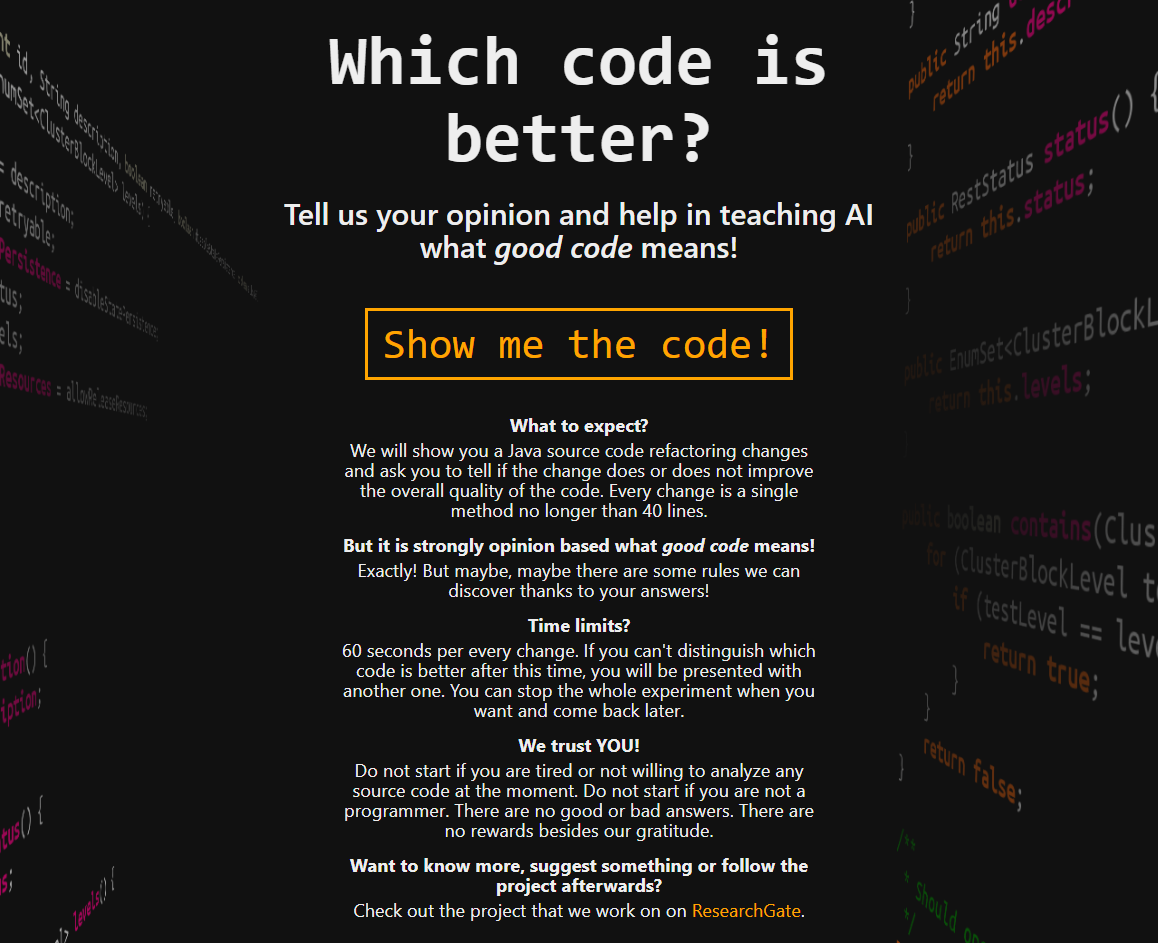
\includegraphics[width=\textwidth]{impl/codefracz-front.png}
\caption{Strona główna platformy stworzonej do zebrania opinii o jakości kodu źródłowego}
\label{fig:impl:codefracz-front}
\end{figure}

\begin{figure}
\centering
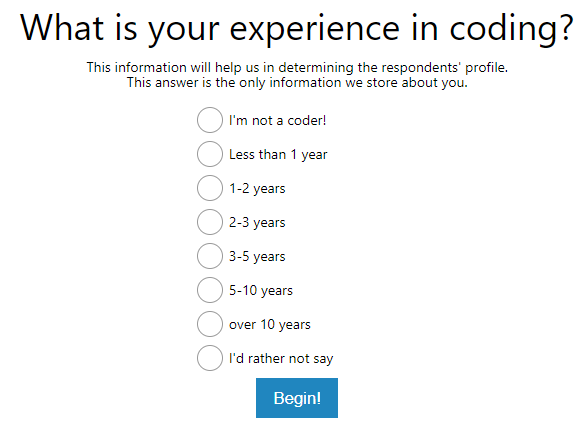
\includegraphics[width=\textwidth]{impl/codefracz-ankieta.png}
\caption{Ankieta wyświetlana respondentom badania opinii o jakości kodu przed oddaniem pierwszego głosu}
\label{fig:impl:codefracz-ankieta}
\end{figure}

\subsection{Rezultat badania}
\textcolor{red}{Ile tego się udało zebrać}

Badanie trwało 6 miesięcy (styczeń - czerwiec 2018). Głównymi respondentami byli studenci III i IV roku studiów Informatyki na wydziale IEiT, AGH. W trakcie zajęć z przedmiotów Technologie Obiektowe oraz Inżynieria Oprogramowania poświęcono 10-15 minut, by zachęcić studentów do udziału w badaniu. Tematem laboratoriów przeprowadzanych w ramach tych przedmiotów była jakość kodu, dlatego taka aktywność doskonale wpisywała się w tok zajęć.

Dodatkowo, sporo klasyfikacji udało się zebrać od użytkowników platformy z zadaniami do nauki systemu kontroli wersji Git - \url{https://gitexerecises.fracz.com}. Jest to jeden z wcześniejszych projektów doktoranta, który zyskał sporą popularność w Internecie tak, że witryna notuje co najmniej kilkanaście unikalnych odwiedzin dziennie. Głównie są to programiści, dlatego wstawienie propozycji pomocy autorowi platformy w jego kolejnym projekcie polegającej na ocenie kilku przykładów refaktoryzacji wydawało się dobrym pomysłem - i rzeczywiście tak było.

Charakterystyka zebranych odpowiedzi została przedstawiona na wspomnianej już wcześniej tabeli \ref{tbl:impl:codefracz-respondents}. Natomiast liczba sklasyfikowanych poszczególnych przykładów została przedstawiona w tabeli \ref{tbl:impl:codefracz-results}.

\begin{table}[t]
\caption{Uzyskane klasyfikacje w badaniu opinii o jakości kodu}
\label{tbl:impl:codefracz-results}
\begin{tabular}{|l|l|}
  \hline 
  Kod przed zmianą jest lepszy & XXX \\ \hline
  Kod po zmianie jest lepszy & XXX \\ \hline
  Zmiana nie wpływa na jakość kodu & XXX \\ \hline
\end{tabular} 
\end{table}

Ciekawym spostrzeżeniem jest fakt, że niektóre zmiany refaktoryzacyjne zostały sklasyfikowane jako "anty-refaktoryzacje". Sporo przykładów zostało odrzuconych jako niezmieniające jakości. Większość z nich - zgodnie z oczekiwaniami - została sklasyfikowana jako "kod po zmianie jest lepszej jakości".

\section{Podsumowanie}
\textcolor{red}{SUM UP tego co wyżej}

\chapter{Przebieg uczenia SCQM}
\label{ch:learn}

\textcolor{red}{Wykresy, wykresy, dużo wykresów! Jakie wyniki były tylko z danych przefiltorwanych, jakie po wprowadzeniu klasyfikacji.}

Kolejnym krokiem w dążeniu do weryfikacji tezy rozprawy jest przekazanie wiedzy zawartej w danych zebranych zgodnie z opisem w rozdziale \ref{ch:impl} do modelu sieci neuronowej zaproponowanego w sekcji \ref{sec:impl:rnn}. Oczywiście, mimo szczerych chęci, tworzony model \gls{scqm} nie dawał od razu zadowalających wyników. W tym rozdziale opisano kolejne próby poprawiania założonego modelu oraz pomysły na przygotowanie danych wejściowych, które w konsekwencji doprowadziły do oczekiwanego rezultatu

\section{Ograniczenie długości metod}
\label{sec:learn:len-limit}
Zgodnie z budową sieci neuronowej opisanej w sekcji \ref{sec:impl:rnn} na wejściu model powinien otrzymać macierz $M:N$, gdzie $M$ to najdłuższy możliwy element na wejściu a $N$ to liczba metod w analizowanym zbiorze. Liczba metod $N$ w pozyskanych danych zgodnie z informacjami zawartymi w sekcji \ref{sec:impl:results} to 60764.

Aby określić wymiar macierzy wejściowej $M$ znaleźć maksymalną długość rozbioru syntaktycznego występującą w zebranych danych. Po automatycznym przeanalizowaniu wybranych metod okazało się, że najdłuższa metoda to 32686. Długość metody rozumiana jest jako maksymalna liczba tokenów w jej rozbiorze syntaktycznym w postaci przed lub po refaktoryzacji.

Zgodnie z założeniami danych wejściowych do sieci neuronowej (zob. \ref{sec:impl:rnn-input}) metody, które są krótsze od najdłuższej metody w zbiorze danych należy dopełnić do końca zerami i razem z macierzą wejściową przekazać także liczby znaczących pozycji w poszczególnych wierszach. Oznacza to, że chcąc przeanalizować cały zbiór danych wejściowych potrzeba około 8GB pamięci operacyjniej (zob. wyliczenie \ref{eq:learn:memory}), nie licząc miejsca koniecznego dla budowy modelu sieci neuronowej oraz innych pomocnicze struktury wykorzystywanych przez TensorFlow.

\begin{equation} \label{eq:learn:memory}
MEMORY = M \cdot N \cdot 4B = 32686 \cdot 60764 \cdot 4B = 7944528416B \approx 7.4GB
\end{equation}

Nawet przy posiadaniu sporych zasobów, analizowanie metod tej długości budzi pewne wątpliwości. Z pewnością długość kilku tysięcy węzłów drzewa \gls{ast} sugeruje wspominany już wcześniej zapachu kodu "Long Method". Nawet jeśli metoda była tak duża przed refaktoryzacją a wykonana zmiana poprawiła tę sytuację, trudno powiedzieć że taka operacja została wykonana na poziomie jednej metody.

Aby lepiej poznać profil zgromadzonych danych, za pomocą skryptu \texttt{8\_token\_lengths\_histogram.php} z repozytorium \cite{fracz:refactor-extractor} zliczono długości zgromadzonych metod. To z kolei pozwoliło na naszkicowanie histogramu przedstawiającego rozkład zebranych wartości - przedstawiono go na Rysunku \ref{fig:learn:histogram-dlugosci}.

\begin{figure}
\centering
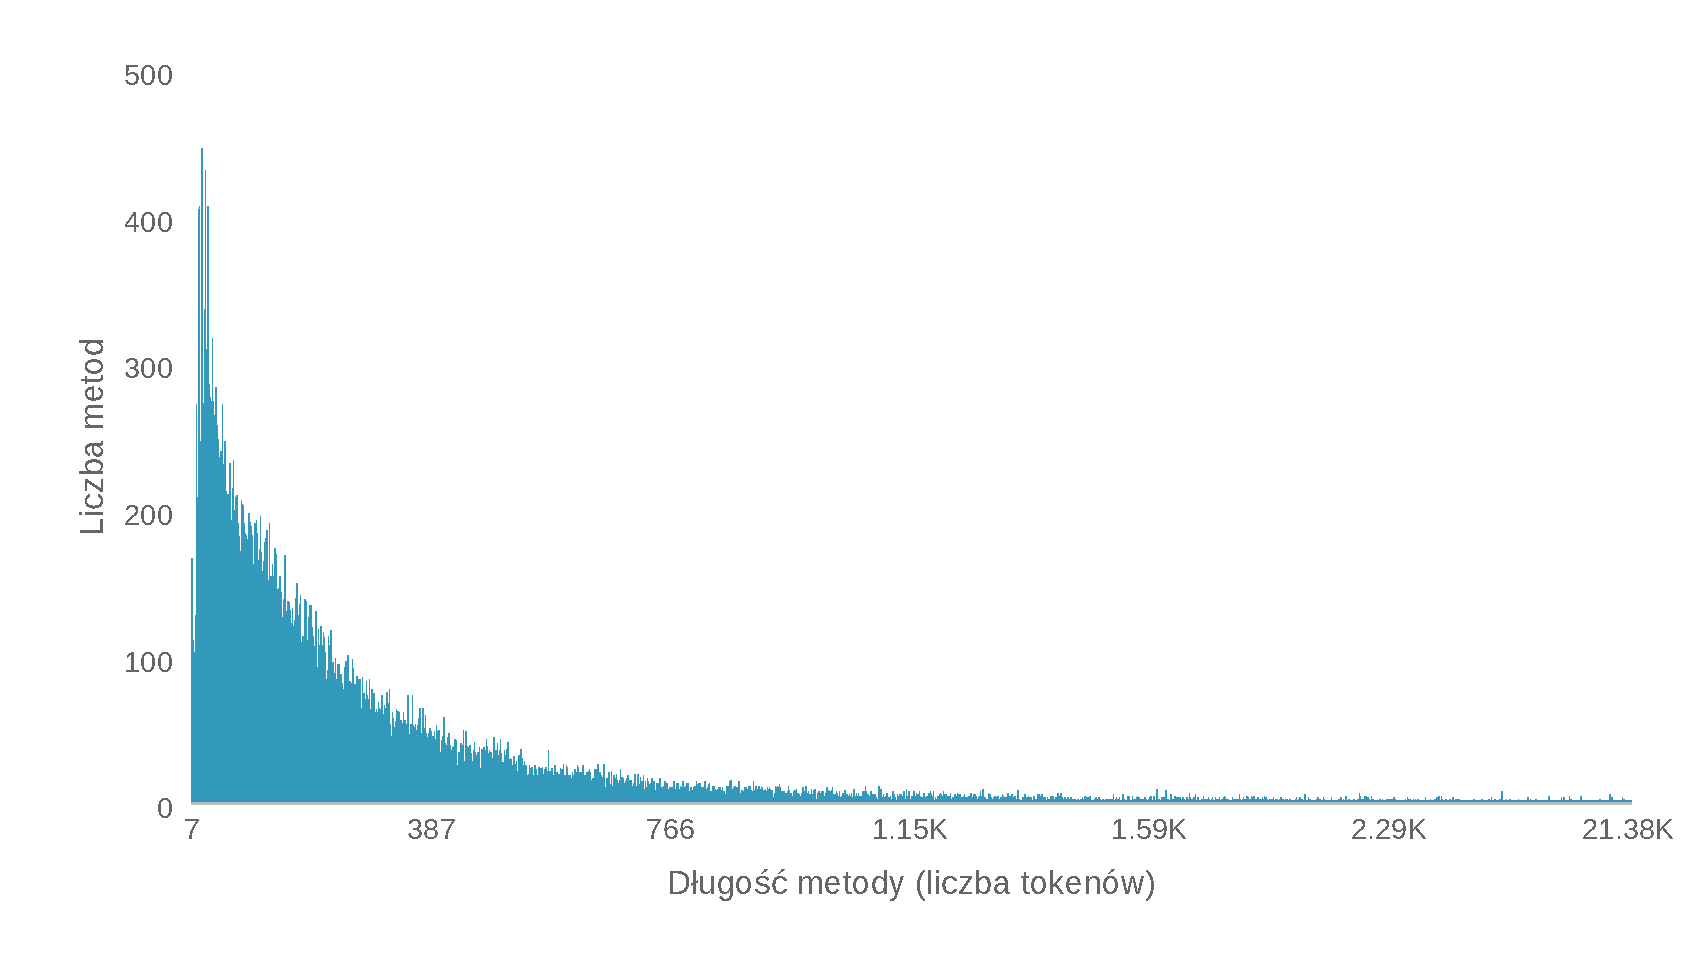
\includegraphics[width=\textwidth]{learn/input-histogram.eps}
\caption{Histogram długości zebranych metod (w tokenach)}
\label{fig:learn:histogram-dlugosci}
\end{figure}

Bez zaskoczenia - przeważająca większość refaktoryzowanych metod jest krótka - dużo krótsza od maksymalnej długości. Moda dla zbioru długości metod jest równa 29, mediana - 168. Te wyniki skłoniły autora rozprawy do znacznego ograniczenia długości metod podawanych na wejściu modelu jeszcze przed pierwszą próbą uczenia.

Aby znaleźć odpowiednią maksymalną długość metody, do której powinno zostać ograniczone wejście, przeanalizowano jaka część zbioru danych pozostaje przy jej zmniejszaniu. W ten sposób oczyszczono zbiór danych z przykładów, które na pewno nie prezentują kodu wysokiej jakości oraz - docelowo - przyspieszono obliczenia modelu. Tabela \ref{tbl:learn:max-len} przedstawia zależność maksymalnej długości metody od liczby próbek, która pozostaje po nałożeniu takiego ograniczenia. Ostatecznie do wstępnych obliczeń przyjęto ograniczenie długości metody do 300 tokenów.

\begin{table}[t]
\caption{Liczba próbek pozostałych w zbiorze danych wejściowych po wprowadzeniu poszczególnych ograniczeń na maksymalną długość metody}
\label{tbl:learn:max-len}
\begin{tabular}{|l|l|l|l|}
  \hline 
  \textbf{Maksymalna długość metody} & \textbf{Liczba pozostałych próbek} & \textbf{Część oryginalnego zbioru wejściowego} \\ \hline
  33000 & 60764 & 100\% \\ \hline
  32000 & 60763 & 100\% \\ \hline
  30000 & 60763 & 100\% \\ \hline
  20000 & 60759 & 100\% \\ \hline
  10000 & 60747 & 100\% \\ \hline
  5000 & 60690 & 100\% \\ \hline
  2000 & 60087 & 99\% \\ \hline
  1000 & 57918 & 95\% \\ \hline
  800 & 56397 & 93\% \\ \hline
  700 & 55254 & 91\% \\ \hline
  600 & 53589 & 88\% \\ \hline
  500 & 51358 & 85\% \\ \hline
  400 & 47910 & 79\% \\ \hline
  300 & 42613 & 70\% \\ \hline
  200 & 34204 & 56\% \\ \hline
  100 & 20226 & 33\% \\ \hline
  50 & 10382 & 17\% \\ \hline
\end{tabular} 
\end{table}

\section{Zbiór testowy}

Obie implementacje modelu - względna i bezwzględna - każdy zbiór wektorów wejściowych dzieliły w stosunku $85\%:15\%$. Większy zbiór stawał się danymi uczącymi (treningoweymi). Drugi zaś - dany testowymi, które nie brały udziału w uczeniu. 

Wszystkie trafności przedstawione w rozprawie zostały oparte o wyniki dla zbioru testowego.

\section{Zasoby obliczeniowe}
\textcolor{red}{Że Prometheus AGH i że dziękujemy i w ogóle. Ile czasu to się uczy na naszych danych. Że było uczone tylko przy użyciu metod ze zbioru uczącego a reszta zostaje na ewaluację. Że zbudowany model dostarczony jest w postaci plików, które potrafi zaimportować TF i za ich pomocą sklasyfikować ztokenizowany kod.}

\section{Początkowe próby - uczenie za pomocą przygotowanych danych}
Dane przygotowane zgodnie z opisem w rozdziale \ref{ch:impl} zostały już wstępnie przefiltrowane. Dodatkowe ograniczenie na maksymalną długość analizowanej metody nałożone zgodnie z opisem w sekcji \ref{sec:learn:len-limit} pozwoliło przypuszczać, że pozostałe rozbiory syntaktyczne metod zawierają całkiem sensowne  refaktoryzacje.

Rezultat uczenia modelu za pomocą uzyskanych danych przedstawiono na rysunku \ref{fig:learn:1st}.

\begin{figure}
\centering
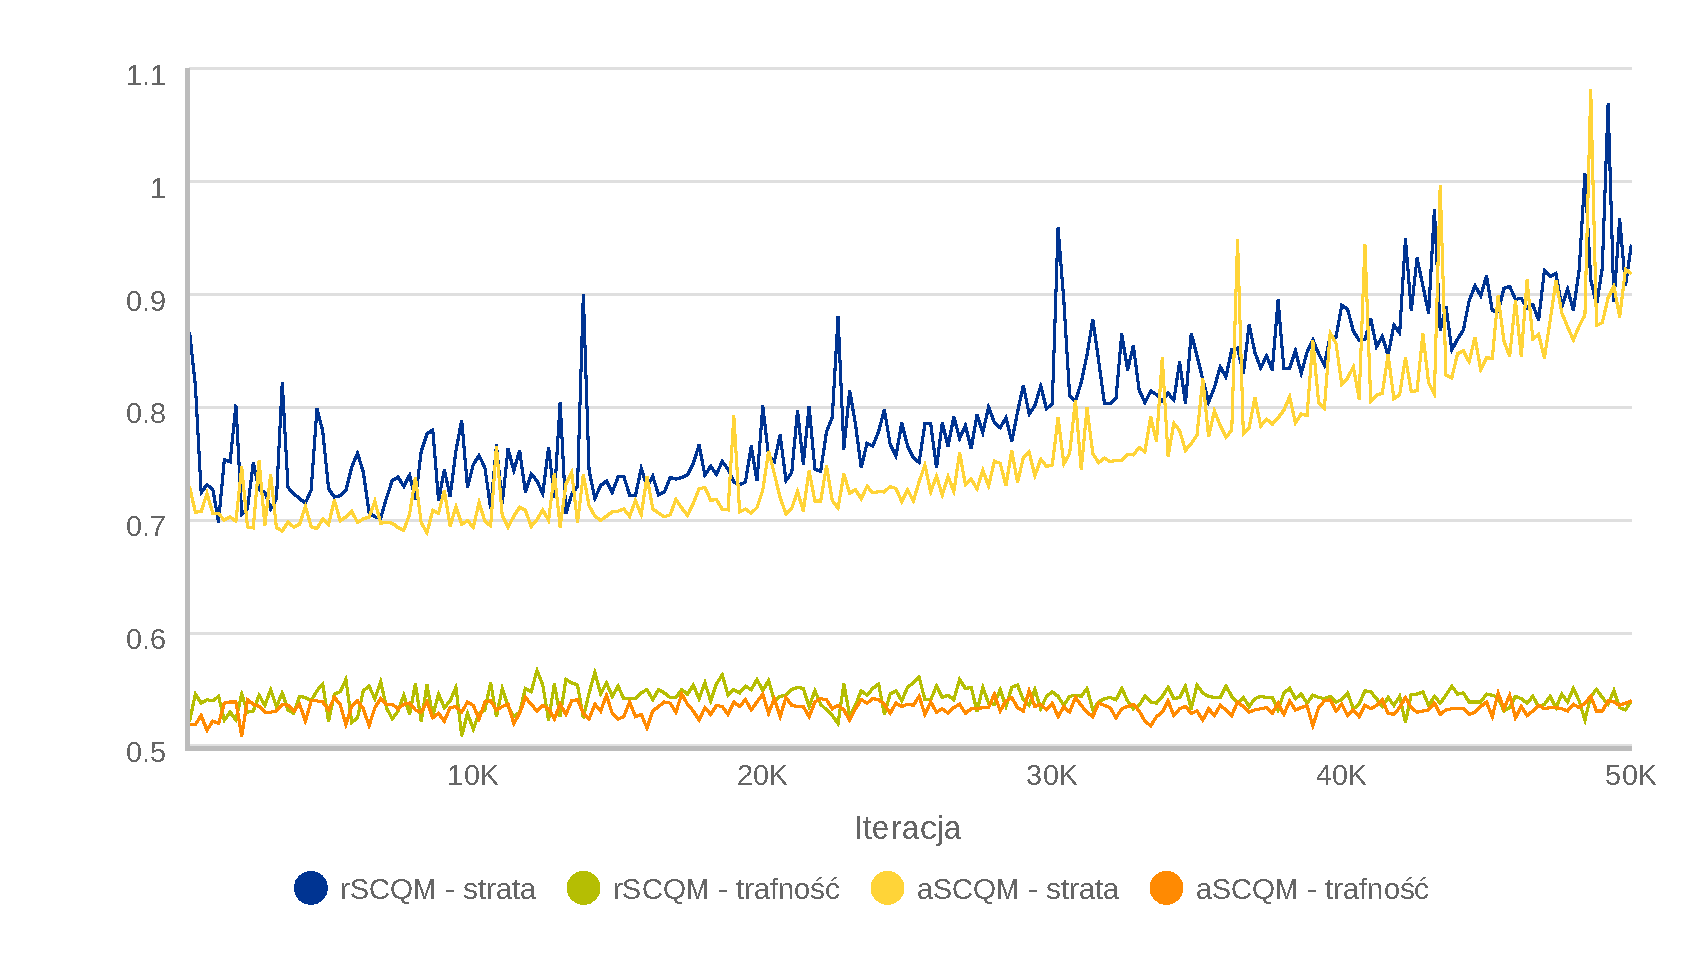
\includegraphics[width=\textwidth]{learn/1st.eps}
\caption{Przebieg pierwszej próby uczenia modelu}
\label{fig:learn:1st}
\end{figure}

Wyniki nie różnią się znacznie od losowej klasyfikacji. Trafność modelu względnego i bezwzględnego po kilkuset pierwszych iteracjach utrzymuje się na poziomie $0.54$. Można zauważyć, że trafność modelu względnego jest odrobinę lepsza, ale zdecydowanie przedstawione wyniki nie są zadowalające.

\section{Testowanie modelu - preparowanie wejścia}
Od samego początku zakładano, że kod przed refaktoryzacją ma niższą jakość niż kod po refaktoryzacji. Tak w rzeczywistości powinno być, ale nawet rezultaty otrzymane z doświadczenia opisanego w sekcji \ref{sec:impl:codefracz} pokazują, że nie zawsze jest to zgodne z prawdą.

Dlatego, po niezadowalających wynikach przy pierwszych próbach uczenia modelu postanowiono sprawdzić, czy zbudowana sieć neuronowa w ogóle jest w stanie przyjąć jakąkolwiek wiedzę z tak zaprojektowanego wejścia.

Podjęto trzy próby stworzenia coraz mniej oczywistej metryki jakości kodu źródłowego i sprawdzono rezultat uczenia na tak przygotowanych danych. Do analizy były wykorzystywane te same metody, które były wybrane w poprzedniej części, ale ich klasyfikacja była przeprowadzona wg zaproponowanych metryk, z porzuceniem zasady "kod przed refaktoryzacją jest niższej jakości niż kod po refaktoryzacji".

W tych testowych próbach modelu ograniczono się do metod o maksymalnej długości 100 tokenów. Zgodnie z tabelą \ref{tbl:learn:max-len}, na wejściu modelu bezwzględnego uzyskano 40452 metody.

\subsection{Negatywne traktowanie wyrażenia warunkowego}

Pierwszą - trywialną - metryką klasyfikującą zebrane metody było negatywne traktowanie wyrażenia warunkowego.

\begin{quotation}
\noindent Jeśli rozbiór syntaktyczny zawiera węzeł \texttt{IfStmt} lub \texttt{ConditionalExpr} - traktuj kod jako niskiej jakości. W przeciwnym razie - traktuj kod jako wysokiej jakości.
\end{quotation}

Wg powyższej reguły 34526 metod zostało sklasyfikowane jako kod niskiej jakości (85\%).

Okazuje się, że dla tak przygotowanych danych model potrzebuje tylko kilkadziesiąt iteracji uczenia by osiągnąć całkowitą skuteczność w rozpoznawaniu przygotowanej definicji kodu niskiej jakości. Przebieg uczenia zaprezentowano na rysunku \ref{fig:learn:fake-ifs}.

\begin{figure}
\centering
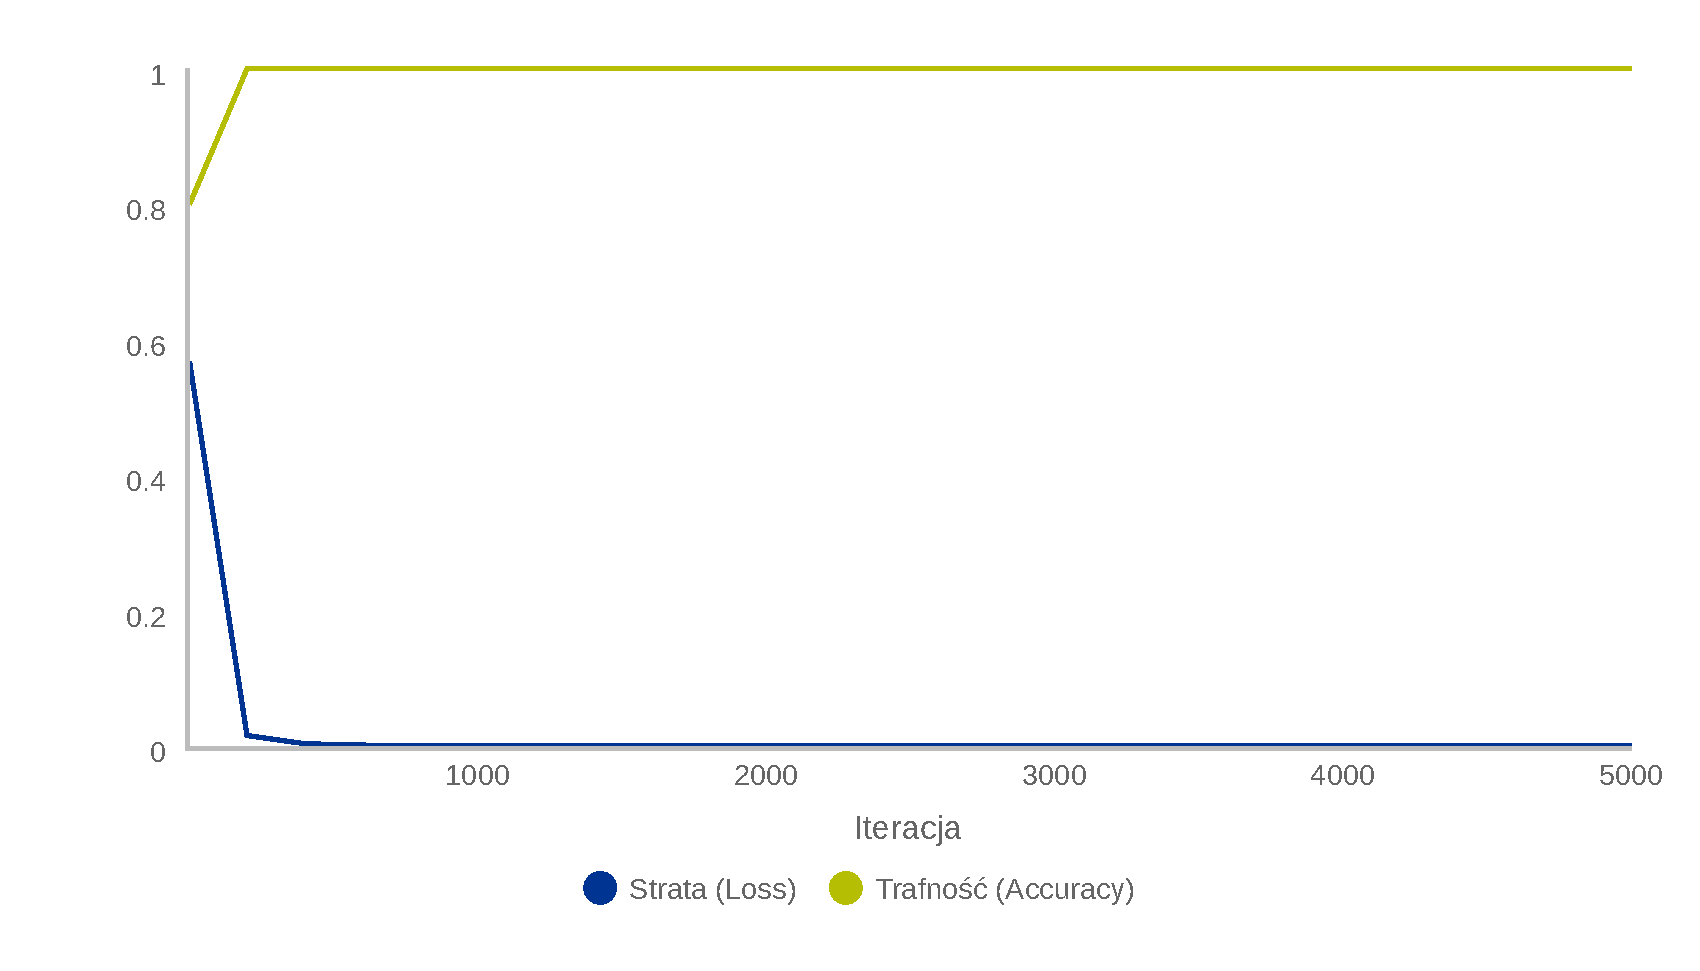
\includegraphics[width=\textwidth]{learn/fake-ifs.eps}
\caption{Rezultat uczenia modelu bezwzględnego w uproszczonej metryce jakości kodu traktującej negatywnie wyrażenia warunkowe}
\label{fig:learn:fake-ifs}
\end{figure}

\subsection{Wirtualna metryka bezwzględna}
\label{sec:learn:fake-static7}
Po uzyskaniu pozytywnego rezultatu przy zastosowaniu trywialnej metryki, podjęto próbę uczenia modelu klasyfikacją wg bardziej złożonej reguły. Wybranym konstrukcjom językowym przypisano koszt (rozumiany jako "koszt zrozumienia danej konstrukcji przez programistę", idąc za przykładem metryki Cognitive Complexity\cite{cognitive}). Ustalone koszty poszczegółnych konstrukcji językowych przedstawiono w tabeli \ref{tbl:learn:fake-cost}.

\begin{table}[t]
\caption{Koszt poszczególnych konstrukcji językowych w przyjętej wirtualnej metryce kodu źródłowego}
\label{tbl:learn:fake-cost}
\begin{tabular}{|l|l|}
  \hline 
  \textbf{Typ węzła \gls{ast}} & \textbf{Koszt} \\ \hline
  \texttt{IntegerLiteralExpr} & 1 \\ \hline
  \texttt{StringLiteralExpr} & 1 \\ \hline
  \texttt{ConditionalExpr} & 2 \\ \hline
  \texttt{ForeachStmt} & 2 \\ \hline
  \texttt{IfStmt} & 2 \\ \hline
  \texttt{CastExpr} & 3 \\ \hline
  \texttt{ForStmt} & 3 \\ \hline
  \texttt{WhileStmt} & 3 \\ \hline
  \texttt{SwitchStmt} & 4 \\ \hline
\end{tabular} 
\end{table}

\begin{quotation}
\noindent Jeśli koszt metody liczony wg tabeli \ref{tbl:learn:fake-cost} przekroczy $7$, traktuj kod jako niskiej jakości. W przeciwnym razie - traktuj kod jako wysokiej jakości.
\end{quotation}

Wartość $7$ ustalono tak, aby reguła podzieliła posiadany zbiór danych w stosunku 40\%:60\%. W efekcie, 17181 metod (42\%) zostało sklasyfikowanych jako kod niskiej jakości.

Wg tak przygotowanych danych, na zbiorze testowym model wahał się bardziej niż przy pierwszej - trywialnej - metryce, ale i tak po kilkudziesięciu iteracjach był w stanie rozpoznać przygotowaną regułę klasyfikacji kodu i jego trafność nie spadała poniżej 98\%. Przebieg uczenia zaprezentowano na rysku \ref{fig:learn:fake-static7}.

\begin{figure}
\centering
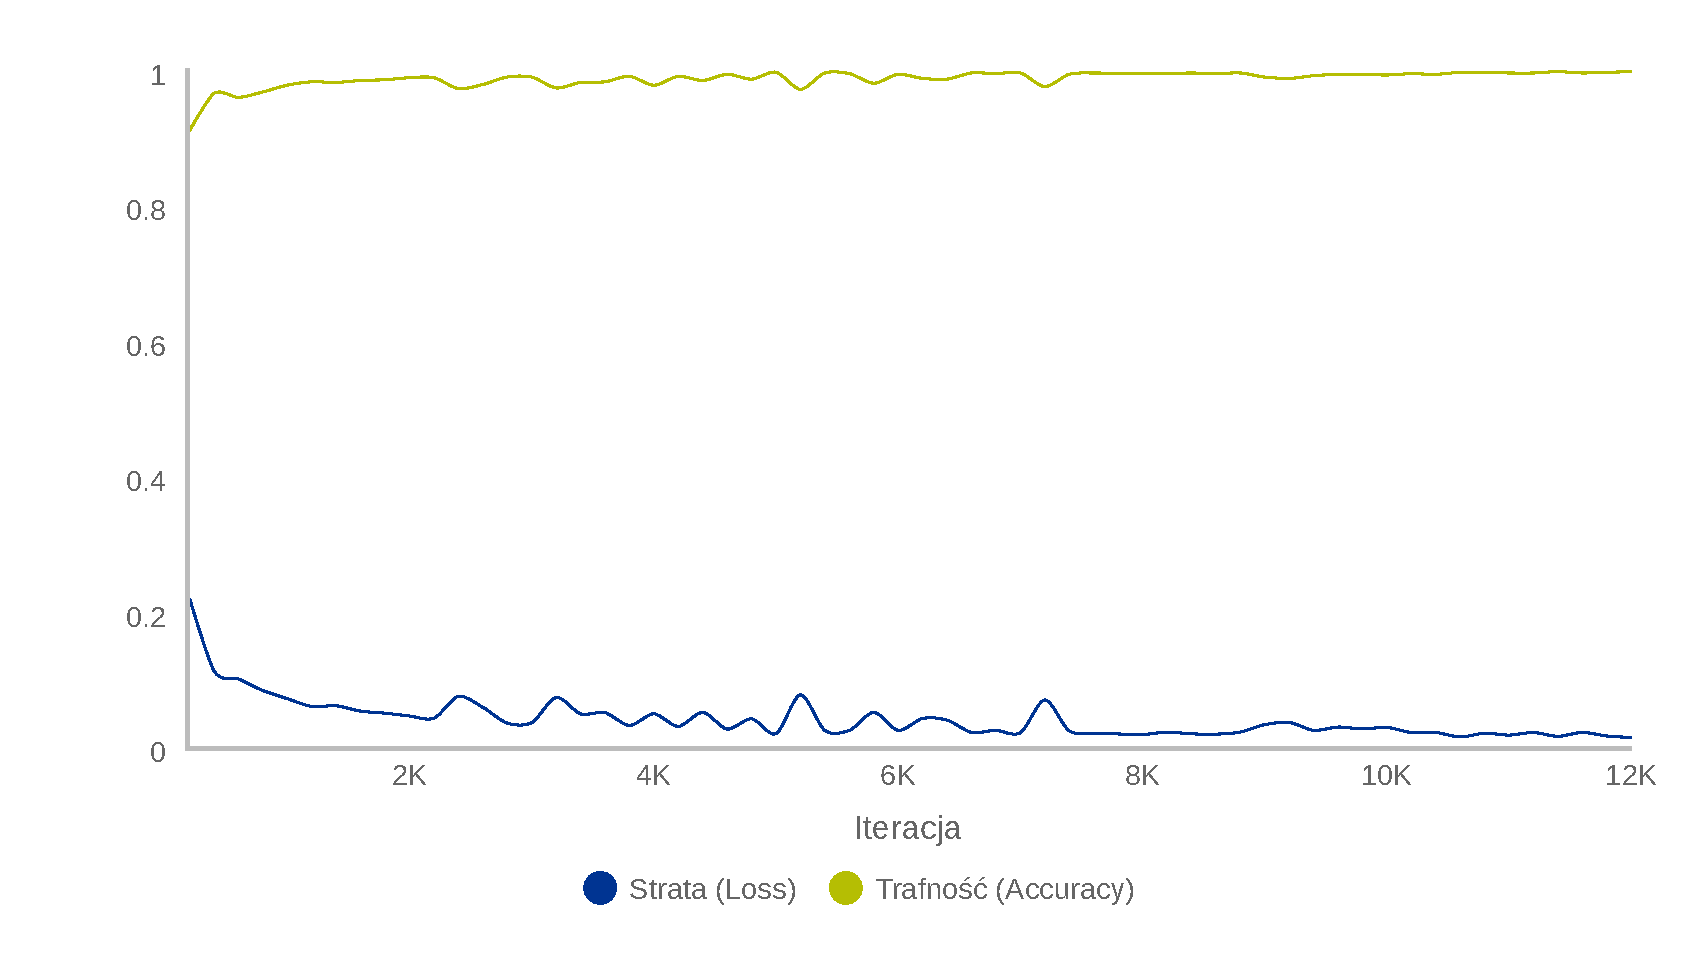
\includegraphics[width=\textwidth]{learn/fake-static-7.eps}
\caption{Rezultat uczenia modelu bezwzględnego w uproszczonej metryce jakości kodu zliczającej koszt wybranych konstrukcji językowych}
\label{fig:learn:fake-static7}
\end{figure}

\subsection{Wirtualna metryka zależna od długości metody}
Metryka zaproponowana w sekcji \ref{sec:learn:fake-static7} nie traktowała sprawiedliwie dłuższych metod. Jeśli metoda posiada 50 konstrukcji językowych, klasyfikacja powinna pozwolić jej na wyższy koszt niż metodzie, która zawiera ich tylko 20. Dlatego finalną metryką rozstrzygająca o poprawnej implementacji modelu sieci neuronowej było uzależnienie kosztu, przy którym metoda była klasyfikowana jako niskiej jakości od jej długości.

\begin{quotation}
\noindent Jeśli stosunek kosztu metody liczonego wg tabeli \ref{tbl:learn:fake-cost} do długości metody wyrażonej w liczbie węzłów \gls{ast} przekroczy $0.15$, traktuj kod jako niskiej jakości. W przeciwnym razie - traktuj kod jako wysokiej jakości.
\end{quotation}

Analogicznie do poprzedniego przypadku - wartość $0.15$ została ustalona empirycznie tak, by uzyskać zrównoważony podział danych wejściowych. Przy zastosowaniu tej reguły, 16533 metody (41\%) zostało sklasyfikowane jako kod niskiej jakości.

Również w tym przypadku model poradził sobie z odpowiednim klasyfikowaniem zbioru testowego. Przebieg uczenia przedstawiono na rysunku \ref{fig:learn:fake-static15}. 

Na tym etapie zakończono testowanie zaimplementowanego modelu i powrócono do prób przekazania wiedzy do modelu na podstawie danych sklasyfikowanych wg oryginalnych założeń.

\begin{figure}
\centering
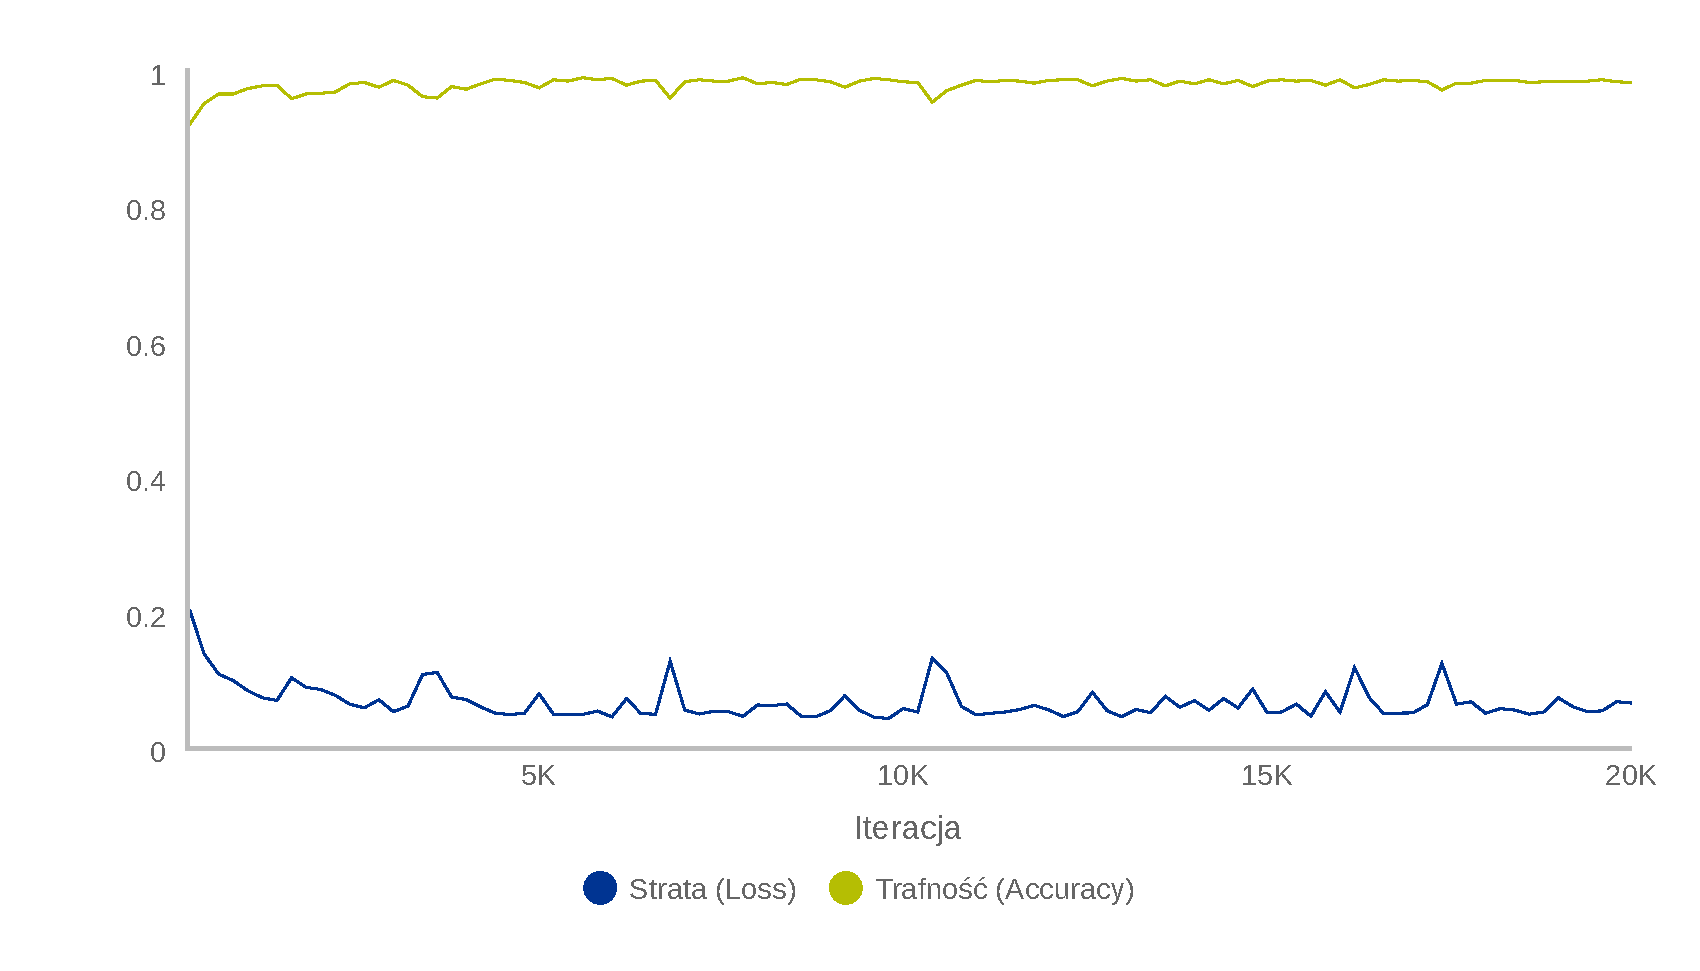
\includegraphics[width=\textwidth]{learn/fake-static-15.eps}
\caption{Rezultat uczenia modelu bezwzględnego w uproszczonej metryce jakości kodu zliczającej wybrane konstrukcje językowe i klasyfikującej kod w zależności od jego długości}
\label{fig:learn:fake-static15}
\end{figure}

Pierwszą próbą poprawy wyników uzyskiwanych przy uczeniu zebranymi danymi i sklasyfikowanymi wg reguły "kod przed refaktoryzacją jest kodem wyżej jakości a kod po refaktoryzacji jest kodem niższej jakości" była zmiana parametrów sieci neuronowej.

\section{Pomysły na usprawnienie uczenia modelu}
\label{sec:learn:better-ideas}
\textcolor{red}{Pomyślano że nie długość ważna ale ile się zmienia, wykluczono pustość itp. Pokaząć co za diff.}

Wszystko wskazywało na to, że dane wejściowe były na tyle niejednoznaczne, że zbudowany model nie był w stanie odkryć w nich żadnych wzorców świadczących o jakości czy czytelności kodu. Jeszcze przed podjęciem decyzji o konieczności zebrania wiedzy ekspertowej (zob. sekcja \ref{sec:impl:codefracz}), postanowiono jeszcze raz przeanalizować zgromadzone metody w nadziei na zidentyfikowanie potencjalnych problemów i jeszcze dokładniejsze przefiltorwanie danych wejściowych dla modelu \gls{scqm}.

\subsection{Zliczanie zmienionych tokenów}

Analizując przypadkowo wybrane przykłady zebranych refaktoryzacji, zwrócono uwagę na powtarzające się sytuacje, których nie wzięto wcześniej pod uwagę, a które pojawiały się w danych wejściowych. Ich jakość byłaby trudna do rozstrzygnięcia nawet przez programistę bez znajomości dodatkowego kontekstu. Niektóre przykłady to:

\begin{enumerate}
\item metody w interfejsach, do których została dodana domyślna implementacja (jest to możliwe od Javy w wersji 8),
\item przeniesienie implementacji w górę hierarchii klas - zastąpienie metody, która dotychczas była abstrakcyjna na metodę nieabstrakcyjną posiadająca implementację,
\item usunięcie całego ciała metody,
\item wykomentowanie lub usunięcie części kodu w ciele metody bez zamiany na np. wywołanie wydzielonej metody prywatnej,
\item dodanie nowego kodu w ciele metody,
\item minimalna zmiana w ciele metody, np. zmiana operatora \texttt{<} na \texttt{<=} w warunku logicznym.
\end{enumerate}

Odkrycie takich przykładów w zebranych przykładach refaktoryzacji odsłoniło potrzebę dokładniejszego ich przefiltrowania. Nie wystarczy, jak założono w sekcji \ref{sec:learn:len-limit}, ograniczyć długości analizowanych metod. Należy także sprawdzić czy kod wewnątrz tych metod rzeczywiście jest \underline{zmieniany}. Należy wykluczyć przypadki, w których kod jest tylko dodawany bądź usuwany. W takiej sytuacji nie tylko programista nie jest w stanie określić, czy kod po danej zmianie jest czytelniejszy, ale także podawanie takiego przykładu w trakcie uczenia modelu bezwględnego wprowadza go w błąd. W ten sposób przy usuwaniu ciała metody model uczy się, że metoda bez ciała jest metodą z kodem wysokiej jakości, a przy dodaniu implementacji - odwrotnie.

W celu przygotowania danych, przetworzono raz jeszcze zgromadzone rozbiory syntaktyczne metod (zob. sekcja \ref{sec:impl:ast}) i na czas przetwarzania umieszczono każdy węzeł drzewa w osobnej linii (zob. skrypt \texttt{15\_prepare\_rnn\_input\_by\_diff.php} z repozytorium \cite{fracz:refactor-extractor}). Następnie porównano tak przygotowane rozbiory syntaktyczne za pomocą prostej implementacji porównywania zawartości ciągów znaków \texttt{Diff}\footnote{\url{http://code.iamkate.com/php/diff-implementation/}}. Wynikiem takiego porównania była tablica, z której każdy element był parą wartości informującą o tym co stało się odpowiednio z danym tokenem przed i po refaktoryzacji. Informacje te zostały przekazane jako stałe

\begin{enumerate}
\item \texttt{Diff::UNMODIFIED} jeśli token przed i po przeprowadzonej zmianie jest niezmieniony,
\item \texttt{Diff::INSERTED}, jeśli token został dodany w trakcie refaktoryzacji,
\item \texttt{Diff::DELETED}, jeśli token został usunięty w trakcie refaktoryzacji.
\end{enumerate}

W celu wyeliminowania niejednoznacznych przykładów wymienionych na początku tej sekcji, ze zbioru danych wejściowych odrzucono przykłady które w wyniku porównania nie zwróciły obydwu stałych oznaczających dodanie lub usunięcie danego tokenu.
 
Ponadto, dla każdej zmiany wyznaczono liczbę zmienionych tokenów, zliczając pary zawierające wartość \texttt{Diff::INSERTED} lub \texttt{Diff::DELETED}. Następnie odrzucono zmiany, które posiadały mniej niż 5 zmienionych tokenów. Po kolejnej weryfikacji przefiltrowanego zbioru danych okazało się, że niektóre ze znalezionych wcześniej negatywnych przypadków refaktoryzacji nadal pozostały w przefiltrowanym zbiorze danych, więc zwiększono minimalną liczbę zmian do 10.

\subsection{Dalsze ograniczanie długości analizowanych metod}

Ponadto, kolejny raz podjęto decyzję o ograniczeniu długości metody do 200, a następnie do 100 tokenów.  Zwrócono bowiem uwagę, że w przypadku zbyt długich metod zmiany w nich przeprowadzane dotyczą często tylko jednego z wielu fragmentów kodu i nawet jeśli jest poprawiana jego jakość - w trakcie uczenia modelu bezwzględnego model będzie źle instruowany o całkowitej jakości kodu. To ograniczenie wydaje się już spore, jednakże 100 tokenów w rozbiorze syntaktycznym metody przekłada się na około 20-30 linii kodu, co wg \textcolor{red}{REF} oraz autora rozprawy i tak jest długą metodą.

\subsection{Pozbycie się nawiasowania z rozbioru syntaktycznego}

W trakcie analizy rozbiorów syntaktycznych metod zwrócono także uwagę, że nawiasowanie tokenów, które zgodnie z sekcją \ref{sec:impl:rnn-input} odzwierciedla strukturę kodu źródłowego, zdecydowanie utrudnia analizę danych wejściowych przez człowieka. Spróbowano więc przygotować zbiór danych wejściowych z pominiętym nawiasowaniem - czyli traktowaniem rozbioru syntaktycznego metody jako płaskiej listy węzłów, które następując jeden po drugim reprezentują przeanalizowany kod źródłowy. W ten sposób tracimy informację o strukturze kodu źródłówego - niemożliwe byłoby odtworzenie kodu na podstawie tak uproszczonego rozbioru syntaktycznego. Autor rozprawy miał nadzieję, że w ten sposób wejście stanie się łatwiej zrozumiałe również dla tworzonego modelu.

Niestety, próba nauczenia modelu tak przygotowanymi danymi dała rezultaty bliskie losowemu klasyfikatorowi, dlatego ostatecznie pomysł z uproszczeniem reprezentacji danych opisanej w sekcji \ref{sec:impl:rnn-input} został porzucony.

\subsection{Zmiana parametrów sieci neuronowej}
\textcolor{red}{Że bawiliśmy się numhidden itp}

W kolejnych próbach uczenia modelu próbowano także zmieniać konfigurację sieci neuronowej zaproponowaną w sekcji \ref{sec:impl:rnn}.

Zmiana parametru prędkości uczenia (ang. learning rate) na mniejszy lub większy nie dawała znaczących zmian w trafności, więc pozostano przy oryginalnym wyborze.

Również zmiana optymizera z Adam na \textcolor{red}{XX lub XX nie dawała zadowalających rezultatów. Przy analizowanym problemie powinien być adam bo REF [XX], dlatego zostawiono Adama. MK help :-(}

\textcolor{red}{Funckja aktywacji to softmax, bo XXXXX więc ją zostawiono MK help :-(}

Jedynym parametrem, który spowodował, że odnotowano zmiany w wynikach uczenia (przy użyciu tych samych danych), była liczba ukrytych warstw \gls{lstm} \textcolor{red}{MK: to chyba nie warsty tylko neurony?}. Liczba ta w teorii reprezentuje liczbę aspekstów, które model jest w stanie wykryć w analizowanych danych. Ile jest aspektów, po których można rozpoznać kod wysokiej jakości? Początkowo wybrano arbitralnie liczbę 128, jednak próba uczenia z większą liczbą ukrytych warstw pokazała, że model zachowuje się lepiej po zwiększeniu tego parametru.

\subsection{Rezultat ponownego filtrowania danych}

Najlepszą kombinacją reguł i parametrów opisanych w tej sekcji okazało się:

\begin{itemize}
\item ograniczenie długości metod do 100 tokenów (20-30 linii kodu)
\item odfiltrowanie zmian, które wyłącznie dodają lub usuwają kod
\item odfiltrowanie zmian, które zmieniają mniej niż 10 lub więcej niż 50 tokenów w rozbiorze syntaktycznym
\item zwiększenie liczby ukrytych warstw \gls{lstm} z 128 do 256
\end{itemize}

Rysunek \ref{fig:learn:diffacc} przedstawia przebieg uczenia modelu dla powyższej kombinacji reguł. Przyjęte nowe reguły filtrowania danych wejściowych pozwoliły poprawić wyniki uczenia o około 10\% dla modelu bezwzględnego.

Tabele \ref{tbl:learn:results-map-bz} i \ref{tbl:learn:results-map-wz} przedstawiają końcową trafność dla zbioru testowego osiąganą po 50 tys. iteracji dla modelu bezwzględnego i względnego dla poszczególnych prób kombinacji.

\begin{figure}
\centering
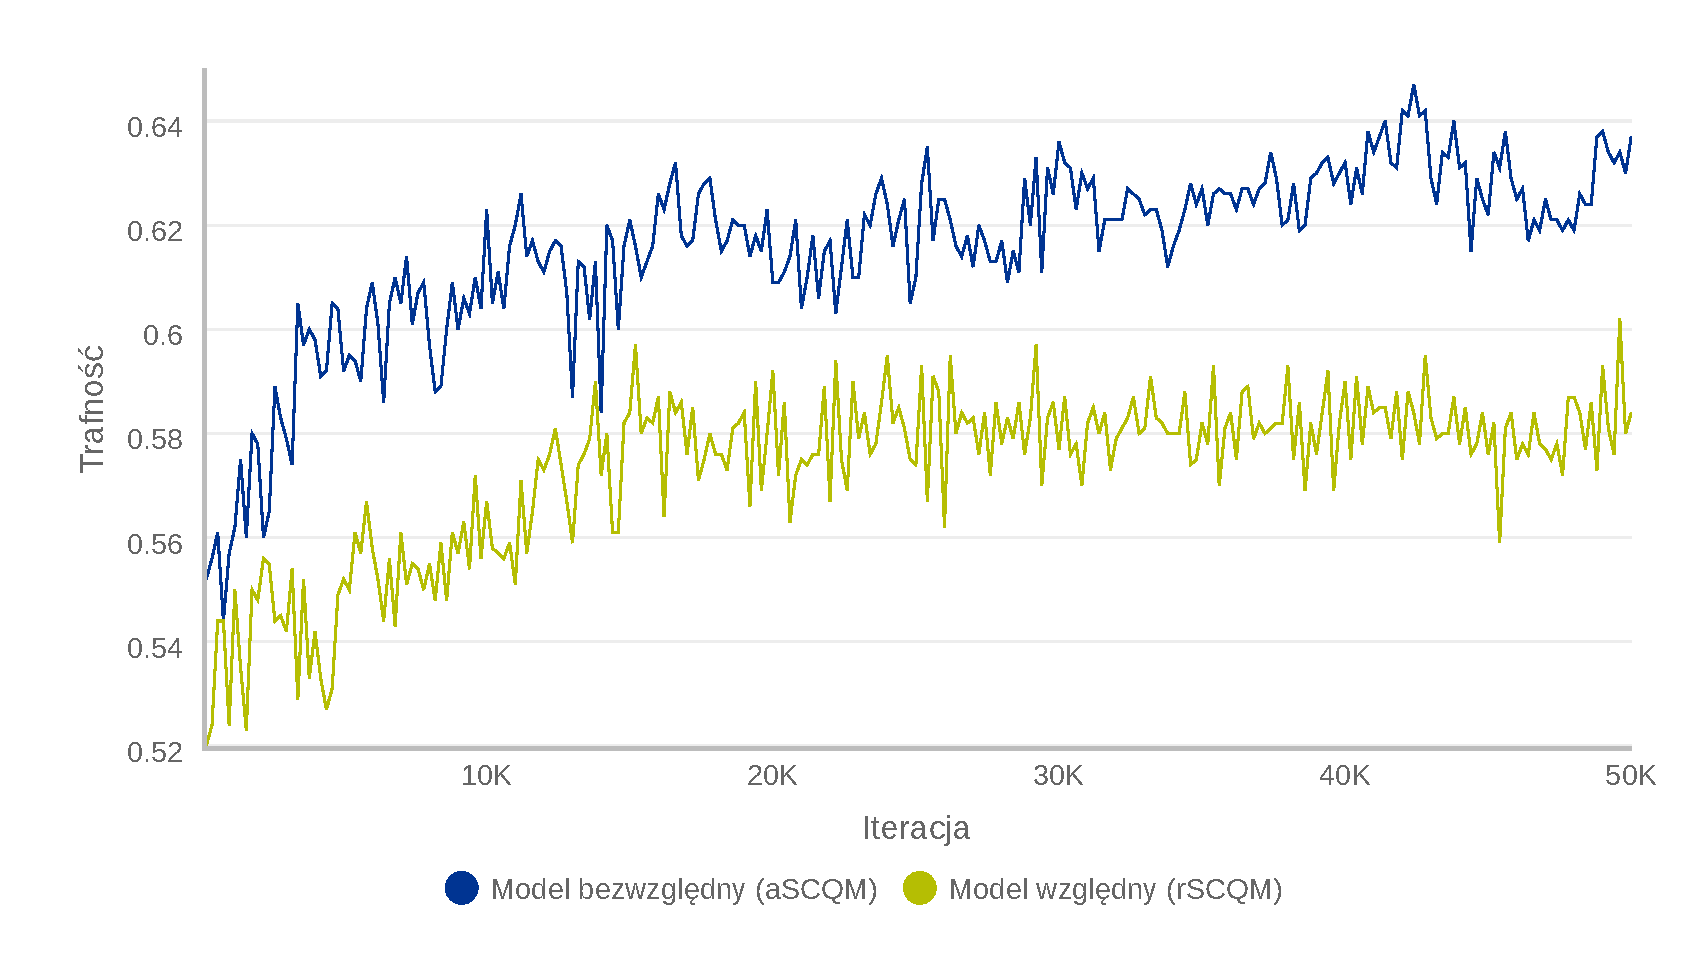
\includegraphics[width=\textwidth]{learn/diffacc.eps}
\caption{Trafność podczas uczenia modelu dla najlepszej uzyskanej konfiguracji parametrów filtrowania danych i sieci neuronowej}
\label{fig:learn:diffacc}
\end{figure}

\begin{table}[t]
\caption{Trafność modelu dla zbioru testowego przy różnych konfiguracjach po 50 tys. iteracji - model bezwględny}
\label{tbl:learn:results-map-bz}
\begin{tabular}{|p{.2\textwidth}|p{.2\textwidth}|p{.2\textwidth}|p{.2\textwidth}|p{.2\textwidth}|}
  \hline 
  \textbf{Maks. długość metody} & \textbf{Min. liczba zmienionych tokenów} & \textbf{Maks. liczba zmienionych tokenów} & \textbf{Liczba ukrytych warstw LSTM} & \textbf{Trafność} \\ \hline 
  300 & - & - & 128 & 53\% \\ \hline 
  200 & 10 & - & 128 & 54\% \\ \hline
  100 & 10 & - & 128 & 58\% \\ \hline
  100 & 10 & - & 256 & 59\% \\ \hline
  100 & 10 & - & 512 & 58\% \\ \hline
  100 & 5 & 100 & 256 & 59\% \\ \hline
  200 & 10 & 50 & 256 & 55\% \\ \hline
  100 & 5 & 100 & 256 & 60\% \\ \hline
  100 & 10 & 50 & 256 & 64\% \\ \hline
\end{tabular} 
\end{table}


\begin{table}[t]
\caption{Trafność modelu dla zbioru testowego przy różnych konfiguracjach po 50 tys. iteracji - model względny}
\label{tbl:learn:results-map-wz}
\begin{tabular}{|p{.2\textwidth}|p{.2\textwidth}|p{.2\textwidth}|p{.2\textwidth}|p{.2\textwidth}|}
  \hline 
  \textbf{Maks. długość metody} & \textbf{Min. liczba zmienionych tokenów} & \textbf{Maks. liczba zmienionych tokenów} & \textbf{Liczba ukrytych warstw LSTM} & \textbf{Trafność} \\ \hline 
  300 & - & - & 128 & 53\% \\ \hline 
  200 & 10 & - & 128 & 54\% \\ \hline
  100 & 10 & - & 128 & 50\% \\ \hline
  100 & 10 & - & 256 & 53\% \\ \hline
  200 & 10 & 50 & 256 & 54\% \\ \hline
  100 & 10 & 50 & 256 & 56\% \\ \hline
\end{tabular} 
\end{table}

Przyjęcie nowych reguł filtrowania danych wejściowych spowodowało kolejne ograniczenie ich liczby. Po nałożeniu nowych warunków na dane wejściowe w zbiorze pozostaje 6821 zmian refaktoryzacyjnych. Porównując tę liczbę do liczby metod o długości do 100 tokenów z tabeli \ref{tbl:learn:max-len} można stwierdzić, że nowe metody filtrowania odrzuciły $\frac23$ analizowanych dotąd zmian jako niejednoznaczne.

\section{Wykorzystanie wiedzy ekspertowej}
\label{sec:learn:expert}
\textcolor{red}{Że liczyliśmy tylko na meodach z code.fracz}
\textcolor{red}{o tym, że uczyłem najpierw samymi danymi z code.fracz.com ale było tego mało i sieć się przeuczała. Dlatego pomysł z uczeniem na niesklasyfikowanych i potem douczenie ekspoertową wiedzą: PUFF! doktorat :-)}

Trafność 64\% w rozpoznawaniu kodu wymagającego refaktoryzacji uzyskana dla modelu bezwględnego jest lepsza niż trafność losowej klasyfikacji. Niemniej jednak, nie można jeszcze na tym etapie mówić o sukcesie prezentowanego modelu. Kolejnym krokiem usprawnienia modelu było więc wykorzystanie wiedzy ekspertowej zebranej przy użyciu platformy opisanej w sekcji \ref{sec:impl:codefracz}.

Pierwszą próbą było nauczenie modelu tylko przy użyciu metod sklasyfikowanych przez programistów jako zmieniające jakość kodu. Tak zbudowany model powinien rzeczywiście posiąść przekazaną w platformie wiedzę na temat jakości kodu.

Przebieg uczenia zaprezentowano na rysunku \ref{fig:learn:expert}. Model bezwzględny \gls{ascqm} nie poprawił się znacząco w stosunku do poprzedniego wyniku po dokładniejszym przefiltrowaniu danych wejściowych. Zdecydowaną poprawę widać jednak w modelu względnym \gls{rscqm}. Dla tak zadanych danych wejściowych osiąga on trafność rozpoznawania zmiany poprawiającej jakość kodu na poziomie 78\%.

\begin{figure}
\centering
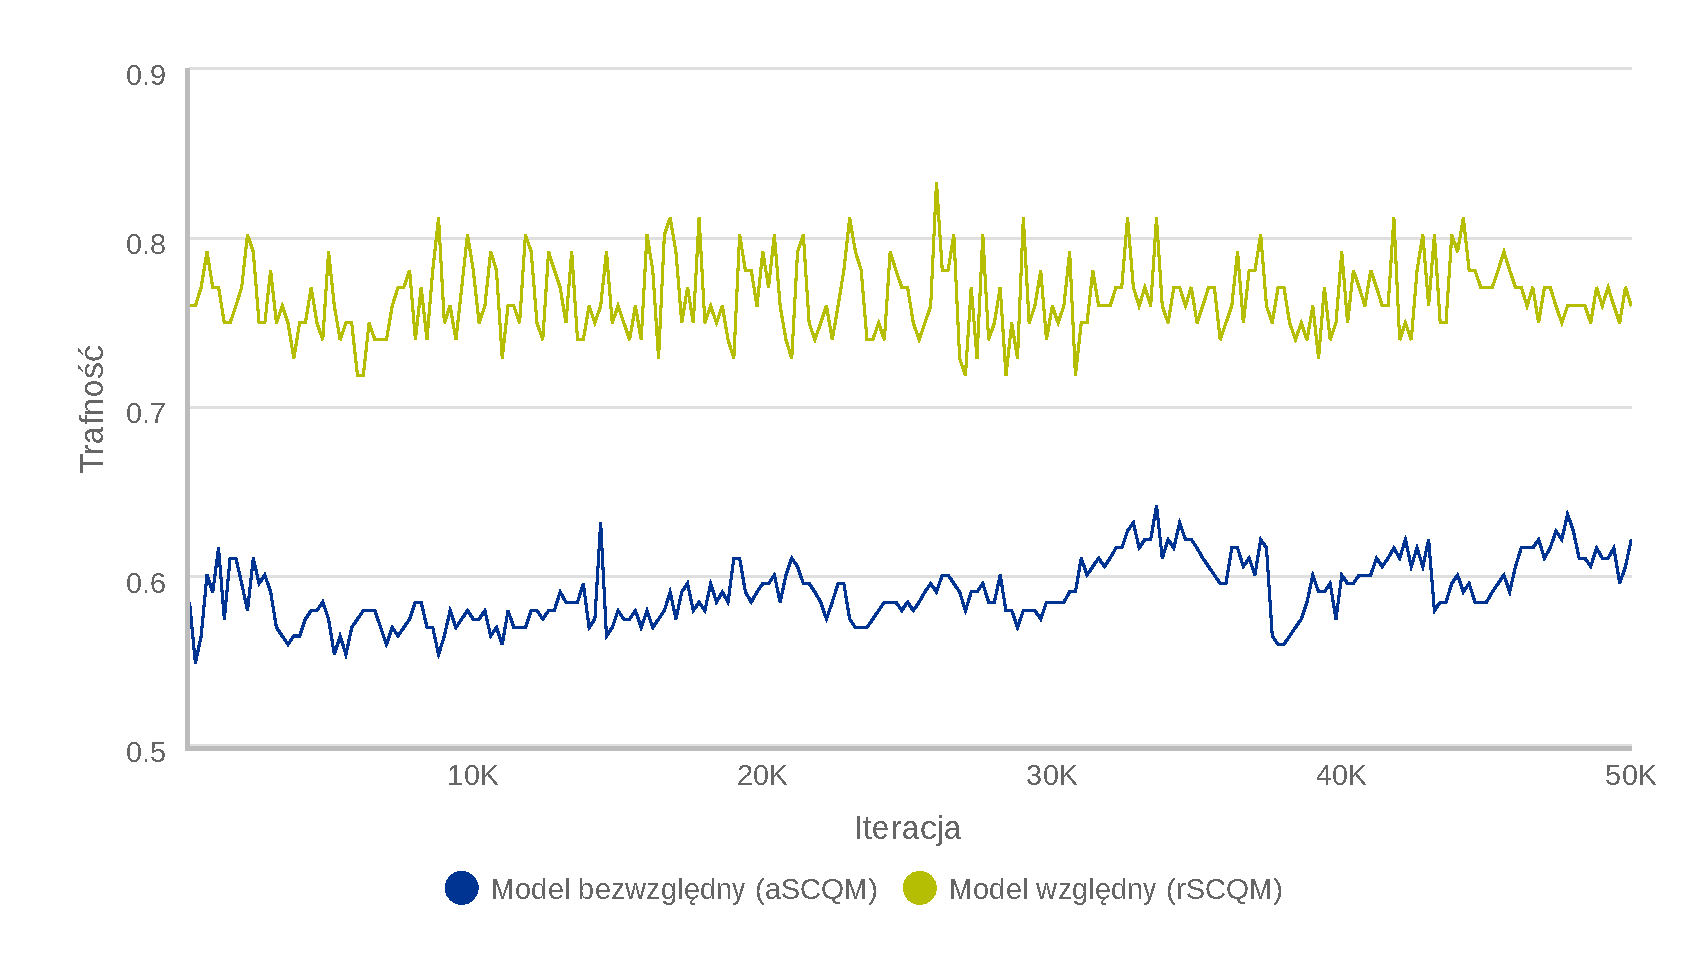
\includegraphics[width=\textwidth]{learn/expert-only.eps}
\caption{Przebieg uczenia modelu przy danych treningowych zbudowanych na podstawie metod sklasyfikowanych przez programistów}
\label{fig:learn:expert}
\end{figure}

\section{Połączenie wiedzy ekspertowej i automatycznie zebranych przykładów}
\textcolor{red}{BAM!}

Ze względu na niewielką liczbę metod sklasyfikowanych przez programistów (zob. Tabela \ref{tbl:impl:codefracz-results}) sieć neuronowa zbyt dobrze dopasowywała się do danych treningowych. Przeuczanie się modelu widać także po szybkim osiągnięciu wysokiej trafności dla modelu \gls{rscqm}.

To doprowadziło do pomysłu połączenia pomysłów opisanych w poprzednich sekcjach \ref{sec:learn:better-ideas} oraz \ref{sec:learn:expert}. W tym wariancie sieć neuronowa jest uczona początkowo za pomocą danych treningowych, które nie zostały sklasyfikowane przez programistów ze względu na ograniczenia eksperymentu.

Pozostając przy dotychczasowym limicie 50 tys. iteracji uczenia ustalono, że model będzie uczony przez 80\% z nich (40 tys.) za pomocą rozbiorów syntaktyczynch metod pozyskanych za pomocą ustalonych reguł opisanych w sekcji \ref{sec:learn:better-ideas}. Następnie, przez kolejne 20\% iteracji (10 tys.), sieć neuronowa zostanie "douczona" poprawnie sklasyfikowanymi metodami przez programistów.

Takie podejście powinno pozostawić w modelu wiedzę o jakości kodu źródłowego wyciągniętą bezpośrednio z otwartych projektów oraz doprecyzować ją za pomocą pozyskanej wiedzy ekspertowej. Aby dokładnie przetestować skuteczność uczenia, w tym podejściu postanowiono stworzyć zbiór testowy złożony wyłącznie z metod sklasyfikowanych przez programistów.

Przebieg uczenia zaprezentowano na wykresie \ref{fig:learn:best-mix}.

\begin{figure}
\centering
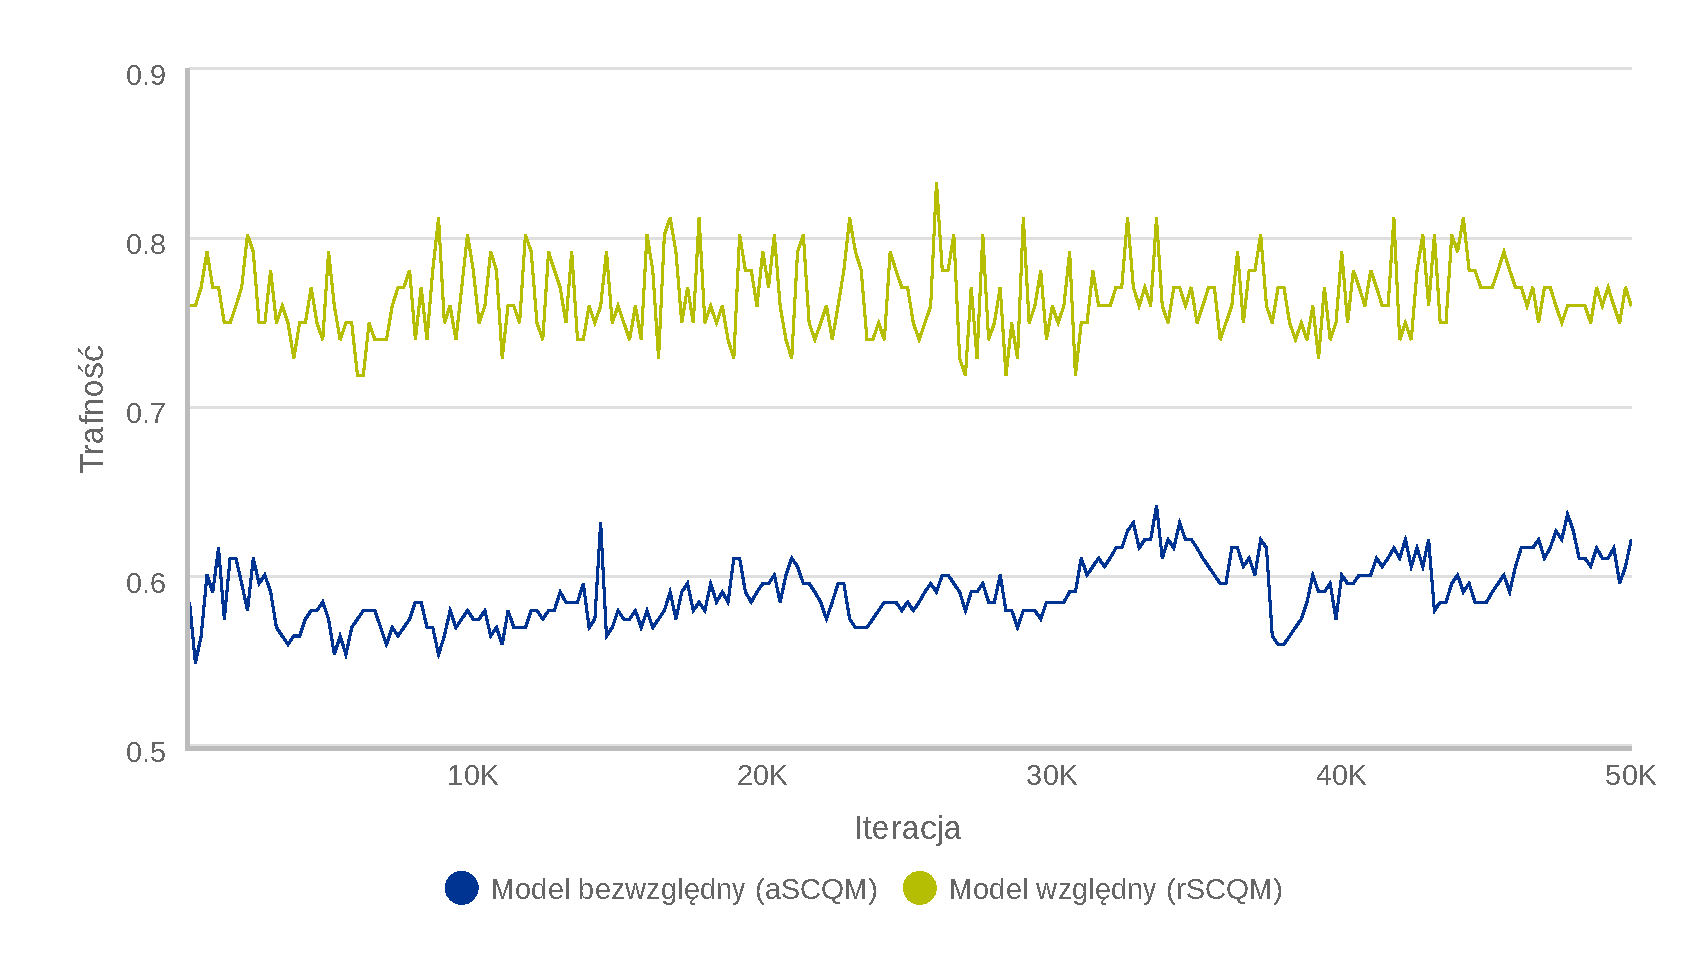
\includegraphics[width=\textwidth]{learn/expert-only.eps}
\caption{Przebieg uczenia modelu przy danych treningowych zbudowanych na podstawie metod sklasyfikowanych przez programistów}
\label{fig:learn:best-mix}
\end{figure}

\section{Podsumowanie}

Kolejne próby uczenia zaprojektowanego jakościowego modelu kodu źródłowego opisane w tym rozdziale pozwoliły na uzyskanie zadowalających rezultatów, a w konsekwencji na kontynuowanie prac nad rozprawą. Proces był najbardziej czasochłonną czynnością w ramach rozprawy ze względu na czas oczekiwania na uzyskanie kolejnych wyników oraz mnogość możliwych rozwiązań.

Na tym etapie uzyskano \textbf{trafność dla modelu \gls{ascqm} na poziomie XX\%} oraz \textbf{trafność dla modelu \gls{rscqm} na poziomie XX\%}. Uznano, że taka trafność uzyskana dla metod sklasyfikowanych w ramach platformy jest wystarczająca, by podjąć próbę porównania stworzonego modelu z istniejącymi narzędziamy oceniającymi kod, opartymi o statyczną analizę.


\chapter{Ewaluacja jakościowego modelu kodu źródłowego}
\label{ch:eval}
\textcolor{red}{Jak już zbudoawłem to teraz zobaczymy jak to się zachowuje.}

\section{Porównywane rozwiązania}
\textcolor{red}{Przedstawienie dwóch innych rozwiązań wspomnianych w related (checkstyle i pmd na przykład) któe oceniają kod i z którymi będę porównywać model. }

\subsection{Reguły klasyfikacji przez porównywane narzędzia}
\textcolor{red}{Przedstawienie reguł np: jak checkstyle lub pmd znajdzie jeden zapach kodu - przyczepi się czegoś - to uważamy że klasyfikuje to jako warte uwagi. Nasz model nie ma reguł, bo od razu ma na wyjściu to co chcemy.}

\section{Wynik porównania}
\textcolor{red}{Tabelki pokazujące że mój model rules the world. Przykłady kodu ewidentnie słabego i pokazanie, że żadne metryki tam nie działają a mój model tak.}

\section{Podsumowanie}
\textcolor{red}{teraz to już na pewno dr inż. Wojciech Frącz}

\chapter{Przykład wykorzystania modelu}
\textcolor{red}{Gamifikacja, gerrit. Nie wiem czy chcę to pisać? Czy mam kłamać że to wprowadziliśmy czy faktycnzie wprowadzić? Może starczy bez tej części i może ją zastąpić podsekcją w podsumowaniu: możliwości czy coś? Mam wrażenie że tak na siłe to tu doklejam. Fajne, podoba mi się, ale nie wiem czy pasuje i czy obecny stan prac pozwala na pisanie o tym.}
% * <dajda@agh.edu.pl> 2018-08-11T13:02:21.956Z:
% 
% wydaje mi się, że to warto to opisać, pytanie tylko czy w tym miejscu. Może warto opisać to gdzieś we wprowadzeniu jako motywacja i możliwości zastosowania? Albo w zakończeniu? Można to zostawić na koniec, zobaczymy ile tego wyjdzie. Ale ponieważ są tutaj ciekawe dane i badania to bym to opisał.
% 
% ^.

\chapter{Wnioski płynące z rozprawy}
\textcolor{red}{Że udało się zbudować model, że udało się zebrać ludzi itp}

\section{Weryfikacja tezy}
\textcolor{red}{Że porównanie wykazało że jest lepiej}

\section{Rozwój pomysłu}
\textcolor{red}{Że można teraz to wdrażać, np hooki w gerricie, gamifikacja (jeśli nie pisałem wcześniej). Że powinno przyspieszyć CR bo nie będziemy skupiać się na pierdołach.}

\clearpage
\addcontentsline{toc}{chapter}{\listfigurename}
\listoffigures

\clearpage
\addcontentsline{toc}{chapter}{\listtablename}
\listoftables

\clearpage
\addcontentsline{toc}{chapter}{\lstlistlistingname}
\lstlistoflistings

\printglossary[title={Akronimy},nonumberlist]

\clearpage
\addcontentsline{toc}{chapter}{Bibliografia}
\bibliography{bibliography}
\bibliographystyle{unsrt}

\end{document}
